En esta sección, extenderemos el número de partículas a $N_{part}=1000$, transformando nuestro choque unidimensional en un gas de particulas interactuantes vía potencial
de Pauli: un \textit{gas de Pauli}.
Como dijimos, nuestro objetivo es confirmar si es posible utilizar este potencial para reproducir las distribuciones de un gas de fermiones no interactuantes (o \textit{gas de Fermi}).

El Hamiltoniano de este gas de Pauli será

\begin{equation}{\label{eq:pauli_gas_ham}}
 H(\mathbf{q}_1, ...,\mathbf{q}_N; \mathbf{q}_1,..., \mathbf{q}_N) = \sum_{i=1}^{N} \frac{p_i^2}{2m} + \sum_{i=1}^N\sum_{j=1}^{i-1} De^{-\frac{1}{2}s_{ij}^2}
 \quad \text{ con } \quad s_{ij}^2 = \frac{|\mathbf{q}_i-\mathbf{q}_j|^2}{q_o^2} + \frac{|\mathbf{p}_i-\mathbf{p}_j|^2}{p_o^2}
\end{equation}

\subsection{Método de simulación}

Con esto en mente, comenzamos extendiendo los algoritmos de la Sección \ref{sec:num_choque_1d} para un sistema de $N$ partículas en 3 dimensiones, con el objetivo
de confirmar si la noción de área excluida se preserva en el límite termodinámico.
En particular, usamos MPR con el método de punto fijo de $k=5$ iteraciones para resolver la ecuación implícita que dicta la evolución temporal del sistema.

Buscamos estimar preliminarmente los tiempos, variando la cantidad de partículas $N$ y analizando el tiempo $\tau_{1000}$ que tardaba el programa en avanzar
$1000$ pasos con $h=5\times10^{-4}$.
Los resultados fueron desalentadores y se encuentran en la \textbf{Figura \ref{fig:tiempo_vs_N}}, donde podemos ver la esperada tendencia cuadrática con
$\tau_{1000} \approx 0.9753\mu s N^{1.988}$.
Esto implica que para $N_{part}=1000$, el programa tardaba $\sim0.86s$ por paso, lo cual resulta simplemente prohibitivo al exigir días de simulación para termalizar el sistema.

\begin{figure}[h]
	\centering
	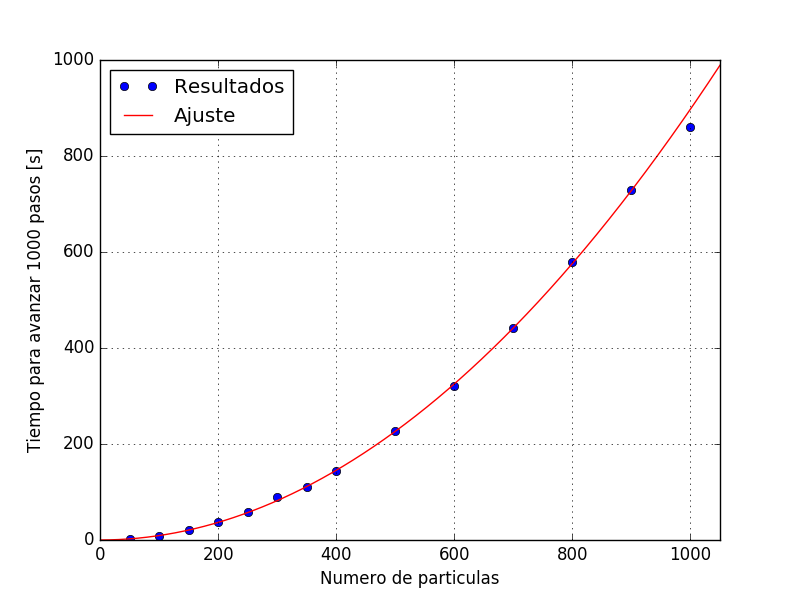
\includegraphics[width=0.6\textwidth]{pauli_gas/tiempo_vs_N.png}
	\caption{Tiempo necesario para avanzar un sistema de $N$ partículas en 1000 pasos con $h=5\times10^{-4}$.
	La tendencia es cuadrática y exige $\sim0.86s$ por paso para $N=1000$, lo cual es prohibitivo.}
	\label{fig:tiempo_vs_N}
\end{figure}

Esto no debería sorprendernos, dado que el método MPR resuelto por punto fijo exige el cómputo de fuerzas $k=5$ veces en total, más del doble de lo exigido por métodos clásicos como Velocity-Verlet.
Además, cabe aclarar que deben computarse las \textit{güerzas} en adición a las fuerzas habituales.
Por último, se suman las complejidades propias del potencial en si, que exige no solo el cálculo de la distancia en el espacio sino también el de la distancia en impulsos y de la necesidad
de computar una exponencial, siempre más costoso computacionalmente que cualquier potencia.

Incluso este $k=5$ resultaba insuficiente a medida que $N$ aumentaba, lo cual es razonable si consideramos que la velocidad de convergencia del método de punto fijo (sección \ref{sec:imp_integs})
depende de $N$ a través de $\nabla^2H$.
De hecho, debió tomarse $h=5\times10^{-4}$ (la mitad que en las simulaciones del choque 1D) para mantener la estabilidad del algoritmo durante estras pruebas, lo cual indirectamente exige una
mayor cantidad de pasos para alcanzar un equilibrio y muestrear propiedades del sistema.

Frente a esto, consideramos más apropiado el uso del método de Metropolis-Montecarlo descripto en \ref{sec:alg_mm} para el Hamiltoniano \eqref{eq:pauli_gas_ham}.
La principal ventaja de este método es que resulta lineal en $N$ dado que el cómputo de $\Delta E$ al modificar la $k$-esima partícula es

\begin{equation}{\label{eq:delta_E}}
 \Delta E =  \frac{|\mathbf{p}_k + \Delta \mathbf{p}|^2}{2m} - \frac{p_k^2}{2m} + \sum_{i=1, i\neq k}^N D\left( e^{-\frac{1}{2}s_{ik}^{'2}}-e^{-\frac{1}{2}s_{ik}^2}  \right)
\end{equation}

Sin embargo, aún avanzando $N$ pasos (en promedio, un intento de movimiento por partícula) este método tardaba aproximadamente $\tau_N = 0.4s$; menos de la mitad.
Esto sumado a la facilidad para controlar la temperatura (dado que nos interesa un sistema NVT), inclinó la balanza en pos de este método.

En lo que sigue, utilizamos el método de Metropolis-Montecarlo para simular una caja de lado $L$ (y volumen $V=L^3$) con $N$ partículas interactuando mediante un potencial de Pauli $V_P$.
Tomamos valores de $\Delta q$ y $\Delta p$ que nos aseguren una aceptación entre $30\%$ y $60\%$.
Estos $\Delta q$ y $\Delta p$ resultan dependientes de la temperatura $T$, la densidad $\rho = N/V = N/L^3$ e incluso de los propios parámetros del Hamiltoniano.
La forma general de estas variaciones fue entonces $\Delta x = x_o f_x(T, \rho, D^*)$  con $x=q,p$.

Además, impusimos una distancia de corte en el espacio de fases $s_{cut}^2=10$ tal que $V_P=0$ si $s_{ij}\geq s_{cut}$.
Esto lo logramos mediante un \textit{shift} del potencial
\[ V_P(s_{ij}^2) = \left\{\begin{matrix} D(e^{-\frac{1}{2}s_{ij}^2}-e^{-\frac{1}{2}s_{cut}^2}) & \text{si } s_{ij}\leq s_{cut} \\ 0 & \text{si } s_{ij}\geq s_{cut} \end{matrix}\right. \]
donde $e^{-\frac{1}{2}s_{cut}^2}\approx 6.7\times10^{-3}\sim 1\%$ del máximo de interacción para $s_{cut}^2=10$.

Tomamos un sistema con condiciones de contorno periódicas (PBC) y utilizamos el criterio de mínima imagen, para lo cual resultaba necesario que el tamaño $L$ de la caja cumpla
\[ L >2 s_{cut}q_o \approx 6.32q_o \]
de forma tal que no sea posible la interacción con más de una imagen simultaneamente.

En lo que sigue, analizaremos propiedades de un gas de Pauli bajo dos conjuntos de parámetros habitualmente utilizados en la literatura para Pauli.
En ambos casos, tomaremos una masa $m=100m_p$ con $m_p=938MeV/c^2$ la masa del protón; un elección arbitraria y, en el fondo, no más que una variación del $D^*$.

El primero de estos conjuntos de parámetros corresponde a Dorso \textit{et al} con
\begin{equation}{\label{eq:params_dorso}}
 \begin{matrix}
  p_o = 2.067 MeV\times 10^{-22}s/fm (= 61.969 MeV/c) & q_o = 6 fm\\
  D = \left(\frac{\hbar}{q_op_o}\right)^3 34.32MeV = \left(\frac{1}{1.88}\right)^3 34.32MeV = 5.165MeV & D^* = 126.16
 \end{matrix}
\end{equation}
y el segundo a Maruyama \textit{et al}
\begin{equation}{\label{eq:params_maruyama}}
 \begin{matrix}
  p_o = 120 MeV/c & q_o = 1.644 fm\\
  D = \left(\frac{\hbar}{q_op_o}\right)^3 207MeV = 207MeV & D^* = 1348.375
 \end{matrix}
\end{equation}

En comparación con \eqref{eq:params_dorso}, los parámetros de \eqref{eq:params_maruyama} generan un potencial de mucho mayor intensidad pero con un alcance mucho mayor en $p$
respecto a su alcance en $q$.
Además, tiene un $D^*$ casi 11 veces mayor, pero tiene un área excluida muy similar
\[ A_M\sim 45\hbar \qquad \text{ vs } \qquad  A_D\sim 28\times1.88\hbar \sim 52\hbar\]
Cualquier diferencia entre ambos, entonces, se deberá a cuestiones morfológicas del área excluida definidas por sus $D^*$ tan distintos.
El resto serán cuestiones de escala definidas por $q_o$ y $p_o$.

Analizamos estos parámetros para 3 densidades distintas, pero dado que el $q_o$ de \eqref{eq:params_dorso} resulta casi 4 veces mayor al de \eqref{eq:params_maruyama}, decidimos mantener
constantes las \textit{densidades reducidas} $\rho^* = q_o^3\rho$.
Elegimos entonces $\rho_o^* = (3/2)^3 = 3.375 $, $\rho_1^* = 1 $ y $\rho_2^* = (1/2)^3 = 0.125 $ representando densidades altas, intermedias y bajas, respectivamente.
Enfriamos estos sistemas desde una $T$ inicial alta (dependiente de $p_o$) donde esperabamos que el sistema se comporte como un gas ideal y enfriabamos sucesivamente para observar los
efectos termodinámicos del potencial de Pauli.

Finalmente, hicimos simulaciones similares para un gas interactuando mediante un potencial de Lennard-Jones (LJ)
\[ V_{LJ}(r) = \varepsilon\left( \left( \frac{\sigma}{r} \right)^{12} - \left( \frac{\sigma}{r} \right)^6 \right) \]
cuya única dependencia proviene de 2 parámetros $\sigma$ y $\varepsilon$, lo cual nos permite facilmente trabajar en unidades reducidas donde $\sigma=1=\varepsilon=m$.
Analogamente, analizaremos las densidades $\rho_{LJ,1}^* = 1.05$ y $\rho_{LJ,2}^* = 0.4$ representando densidades altas y bajas, respectivamente.

Elegimos estas densidades en base al conocido diagrama de fases del potencial de Lennard-Jones, que nos aseguran que corresponden a gas+líquido, líquido+sólido y sólido.

\begin{figure}[h]
	\centering
	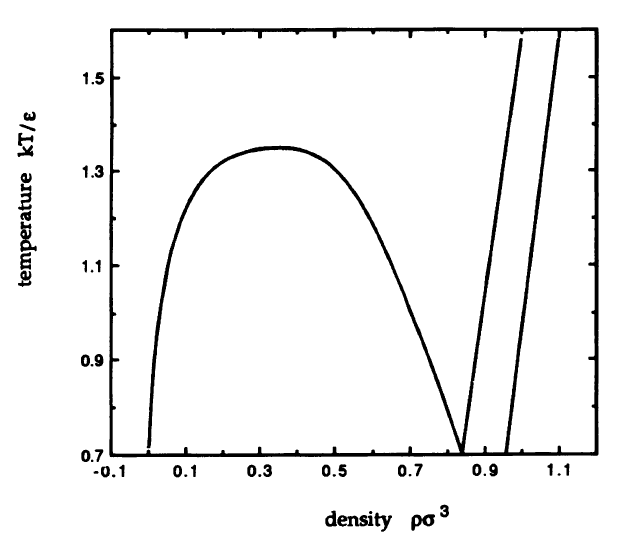
\includegraphics[width=0.4\textwidth]{pauli_gas/phase_diagram_LJ.png}
	\caption{Diagrama de fases de un gas interactuando mediante Lennard-Jones.
	Esto nos asegura que las densidades elegidas $\rho_{LJ,1}^* = 1.05$ y $\rho_{LJ,2}^* = 0.4$ corresponden a líquido+sólido y gas+líquido.}
	\label{fig:ej_diag_fases_LJ}
\end{figure}

Usaremos estas simulaciones a modo de control, para poder apreciar mejor la fenomenología introducida por el potencial de Pauli.

El enfriamiento se realizó reduciendo la temperatura por etapas, esperando a que termalizara en la nueva temperatura y posteriormente muestreando el estado
$(\mathbf{q}_1, ..., \mathbf{q}_N;\mathbf{p}_1, ..., \mathbf{p}_N)$ del sistema (las $6N$ coordenadas).
Este proceso de enfriamiento+muestreo se realizó 8 veces en total, inicializando distintas semillas, para tener una mayor cantidad de muestras y mayor descorrelación entre ellas.
En total, se tomaron $200\times 8 = 1600$ muestras del sistema para cada temperatura.
Sin más preambulos, a continuación se encuentran los resultados.


\subsection{Area excluida}

La propiedad más relevante del potencial de Pauli es la región excluida que estudiamos en el choque unidimensional en la seccion \ref{sec:choque1D}.
Esto, sin embargo, fue para un sistema de $N=2$ partículas y una única dimensión.
Resulta razonable entonces preguntarse si los resultados de la sección \ref{sec:choque1D} siguen siendo válidos.

Como dijimos, esperamos que el potencial de Pauli genere elipsoides $6D$ en el espacio de fases alrededor del $(\mathbf{q}_i,\mathbf{p}_i)$ de cada partícula.
Esto implica que ninguno de los $N(N-1)/2$ $\Delta \mathbf{y}_{ij} = (\Delta \mathbf{q}_{ij}, \Delta \mathbf{p}_{ij}) = (\mathbf{q}_i-\mathbf{q}_j,\mathbf{p}_i-\mathbf{p}_j)$ caerán dentro
de una región centrada en el origen de coordenadas.

Para simplificar esto y evitar trabajar con las 6 dimensiones de estos vectores $\Delta \mathbf{y}$, podemos aprovechar que este elipsoide debería ser simétrico ante rotaciones en $\mathbf{q}$
y en $\mathbf{p}$ por separado, por lo que nos bastan 2 magnitudes para caracterizarlo.
Esta simetría nos permite analizar la región excluida mediante los $\Delta y_{ij} = (\Delta q_{ij},\Delta p_{ij}) \equiv (|\Delta \mathbf{q}_{ij}|, |\Delta \mathbf{p}_{ij}|)$, volviendo
unidimensional nuevamente este problema.
En este caso, dado que usamos el criterio de mínima imagen a la hora de calcular las interacciones, lo usaremos también para calcular las distancias $\Delta q$, por lo que ningún
par de partículas se alejará más de $\sqrt{3}L/2$.

Esta formulación hubiera sido válida (aunque poco natural) para el caso del choque unidimensional de \ref{sec:choque1D}, donde veriamos solo el cuadrante superior derecho de los diagramas de
fases como el de la \textbf{Figura \ref{fig:ej_diag_fases}}.
Esto implica que hay un factor $4$ relacionando las áreas de las regiones excluidas consideradas de una u otra forma.

Tomando las distribuciones de las 8 repeticiones realizadas, hicimos un histograma 2D de los $(\Delta q_{ij},\Delta p_{ij})$ para cada $\rho^*$ y conjunto de parámetros.
Seleccionamos 2 de estas densidades $\rho^*$ y algunas temperaturas para mostrar en las \textbf{Figuras \ref{fig:exclusion_dorso}} y \textbf{\ref{fig:exclusion_dorso}} los histogramas
para los parámetros de Dorso y Maruyama, respectivamente.
Más allá de la diferencia en escalas (que analizaremos en mayor profundidad en \ref{sec:dist_energ}), vemos que ambos conjuntos de parámetros a $T$ baja presentan una región elíptica alrededor
del origen totalmente despoblada.
Al aumentar la temperatura, esta región parece desaparecer progresivamente.

\begin{figure}[H]
	\centering	%trim={<left> <lower> <right> <upper>}
	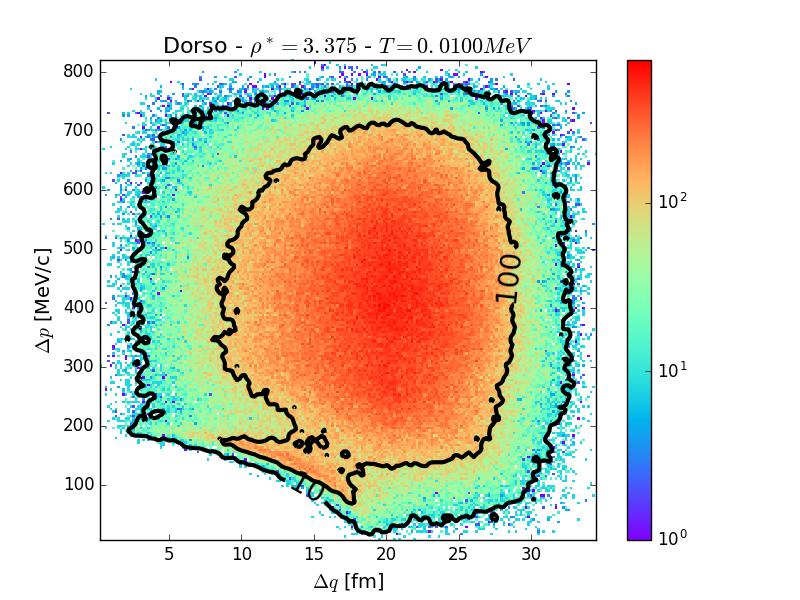
\includegraphics[trim = 5mm 0mm 50mm 5mm, clip, height=0.3\textwidth]{pauli_gas/exclusion/exclusion_rho0_dorso_0,01.png}
	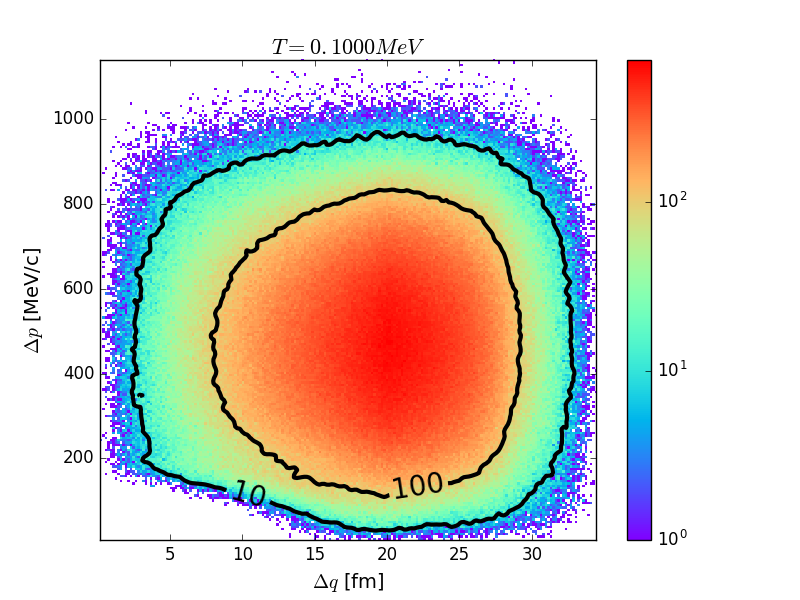
\includegraphics[trim = 14mm 0mm 50mm 5mm, clip, height=0.3\textwidth]{pauli_gas/exclusion/exclusion_rho0_dorso_0,1.png}
	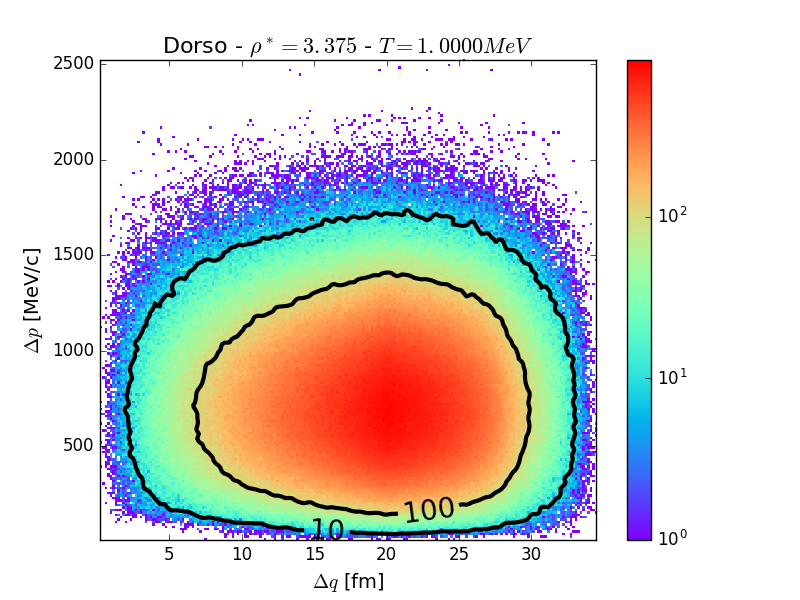
\includegraphics[trim = 12mm 0mm 20mm 5mm, clip, height=0.3\textwidth]{pauli_gas/exclusion/exclusion_rho0_dorso_1.png}
	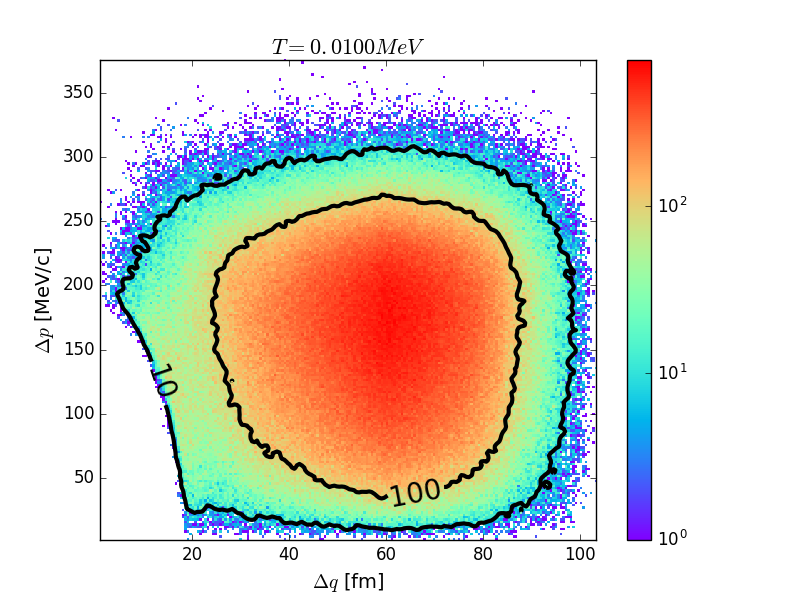
\includegraphics[trim = 5mm 0mm 50mm 5mm, clip, height=0.3\textwidth]{pauli_gas/exclusion/exclusion_rho2_dorso_0,01.png}
	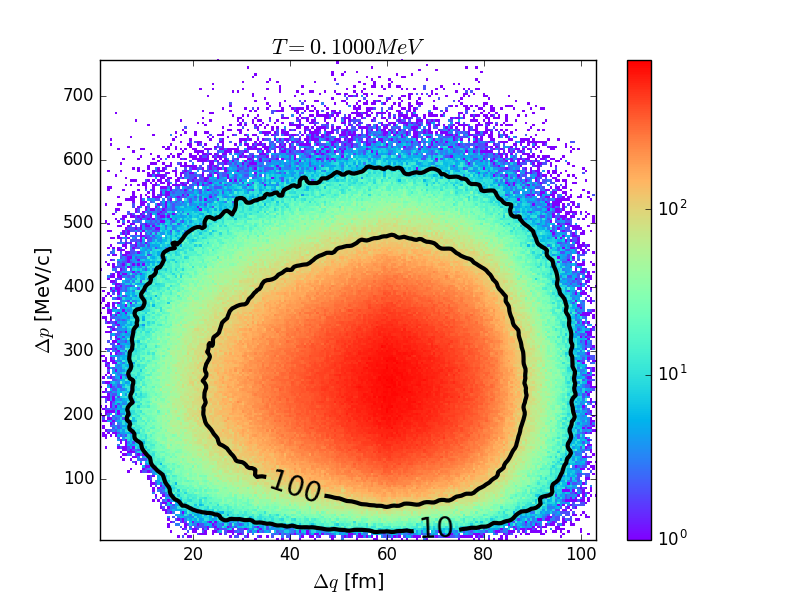
\includegraphics[trim = 15mm 0mm 50mm 5mm, clip, height=0.3\textwidth]{pauli_gas/exclusion/exclusion_rho2_dorso_0,1.png}
	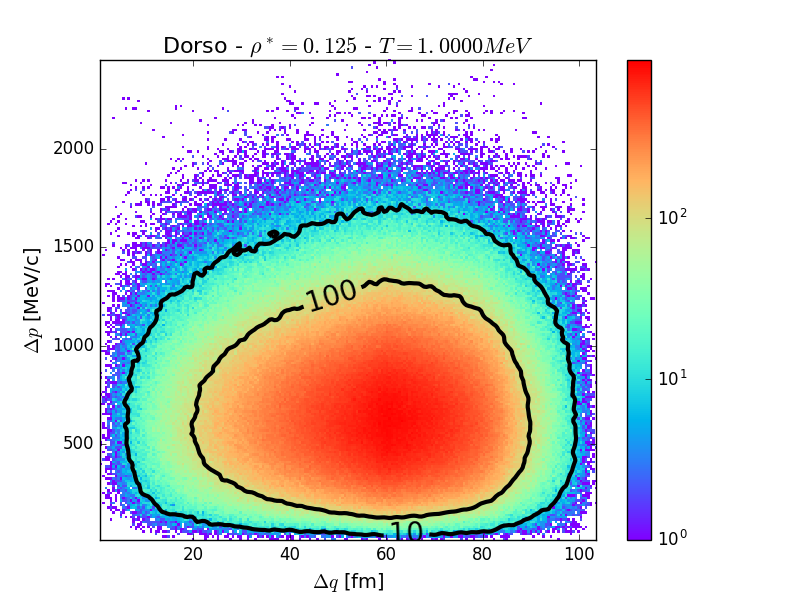
\includegraphics[trim = 12mm 0mm 20mm 5mm, clip, height=0.3\textwidth]{pauli_gas/exclusion/exclusion_rho2_dorso_1.png}
	\caption{Ocupación del espacio de fases $(\Delta q, \Delta p)$ para los parámetros de Dorso y las dos densidades extremas $\rho^*=0.125$ (baja) y $\rho^*=3.375$ (alta).
  Para temperaturas bajas, se evidencia la existencia de una región excluida.}
	\label{fig:exclusion_dorso}
\end{figure}
\begin{figure}[H]
	\centering	%trim={<left> <lower> <right> <upper>}
	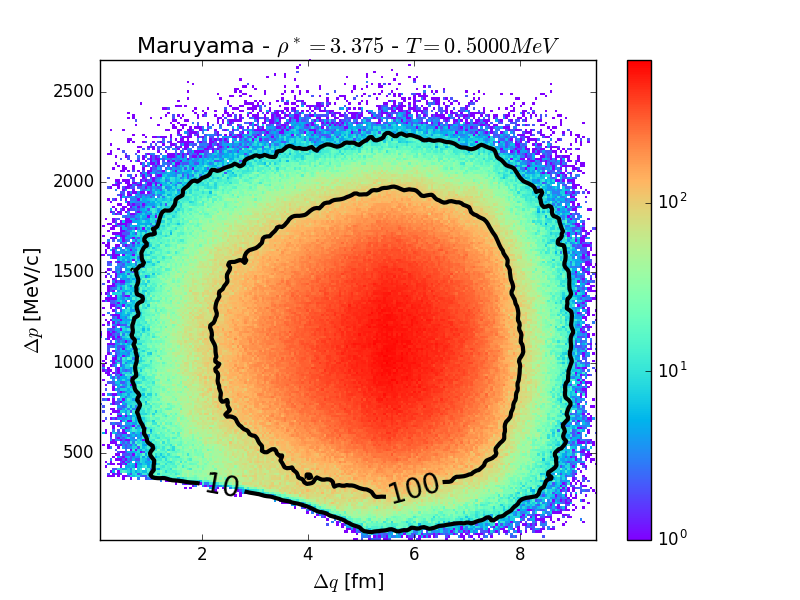
\includegraphics[trim = 5mm 0mm 50mm 5mm, clip, height=0.3\textwidth]{pauli_gas/exclusion/exclusion_rho0_maruyama_0,5.png}
	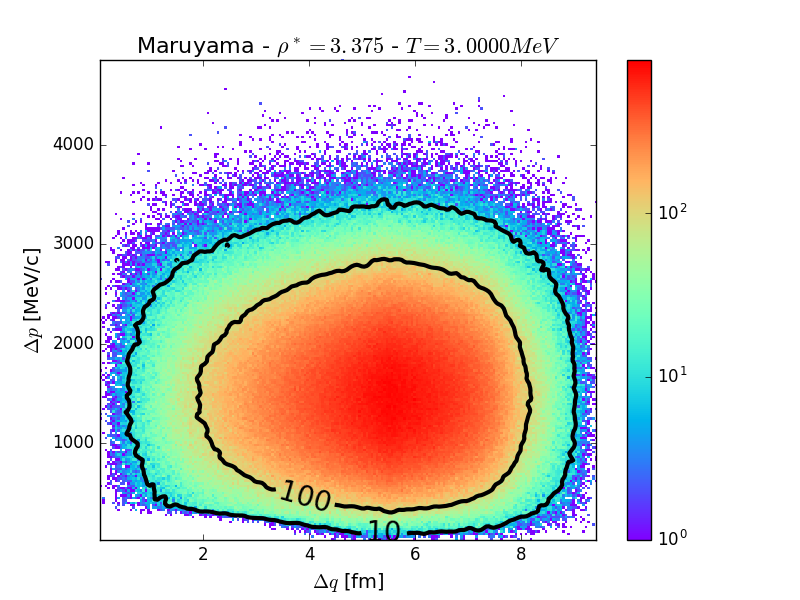
\includegraphics[trim = 14mm 0mm 50mm 5mm, clip, height=0.3\textwidth]{pauli_gas/exclusion/exclusion_rho0_maruyama_3.png}
	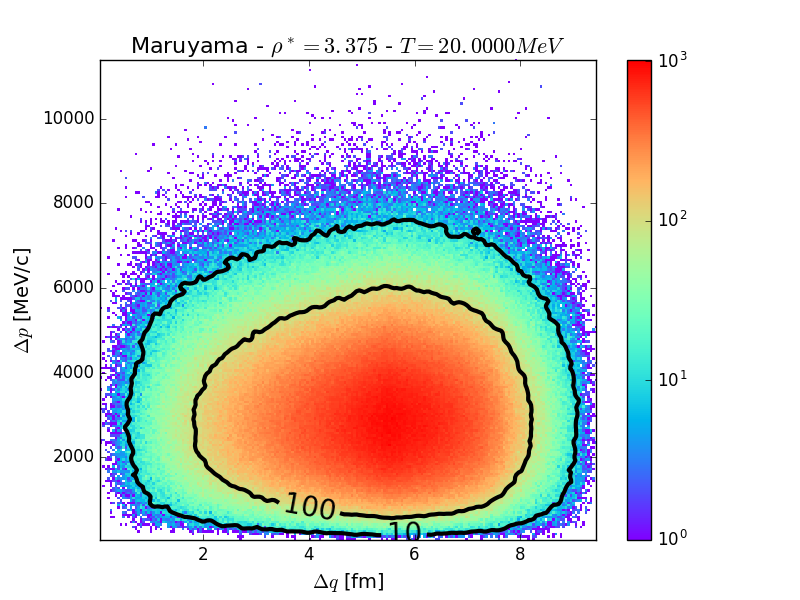
\includegraphics[trim = 12mm 0mm 20mm 5mm, clip, height=0.3\textwidth]{pauli_gas/exclusion/exclusion_rho0_maruyama_20.png}
	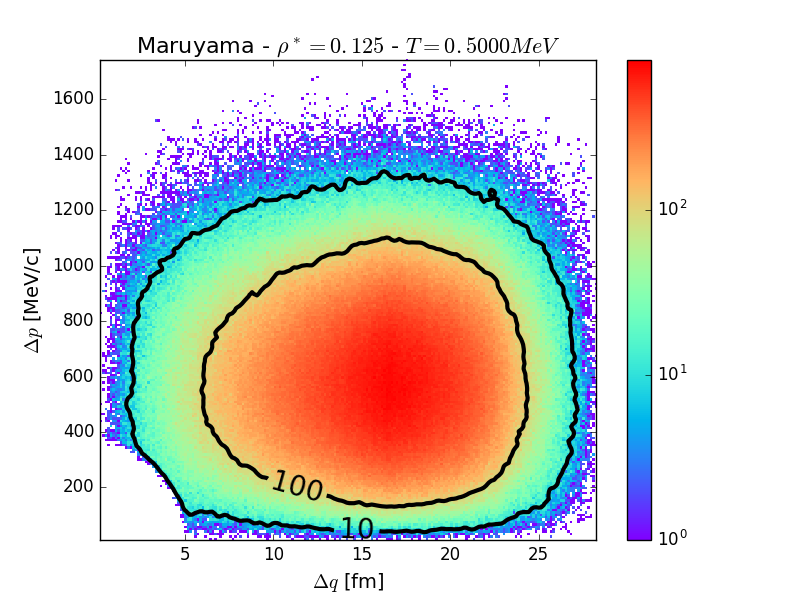
\includegraphics[trim = 5mm 0mm 50mm 5mm, clip, height=0.3\textwidth]{pauli_gas/exclusion/exclusion_rho2_maruyama_0,5.png}
	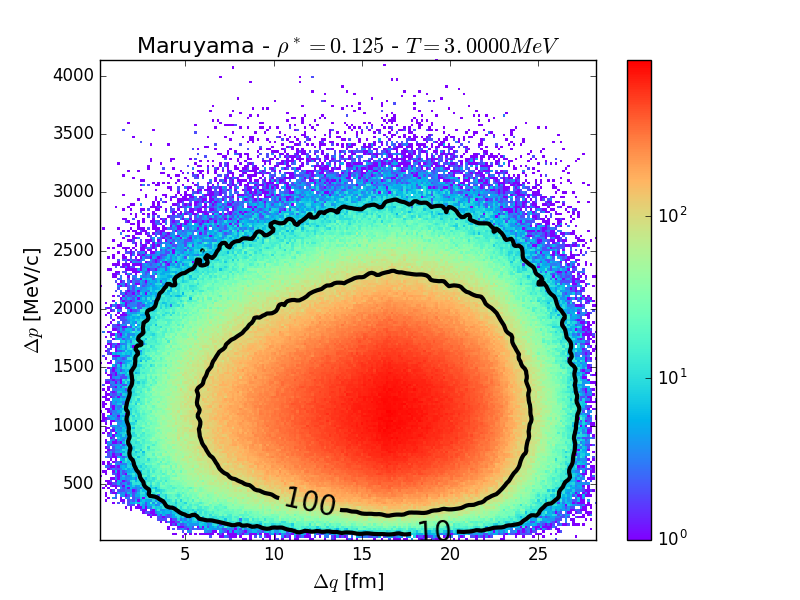
\includegraphics[trim = 15mm 0mm 50mm 5mm, clip, height=0.3\textwidth]{pauli_gas/exclusion/exclusion_rho2_maruyama_3.png}
	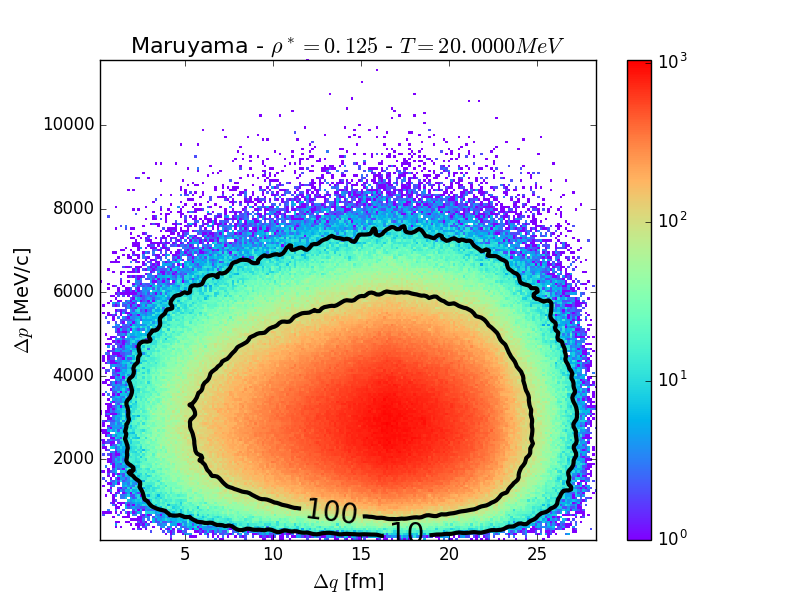
\includegraphics[trim = 12mm 0mm 20mm 5mm, clip, height=0.3\textwidth]{pauli_gas/exclusion/exclusion_rho2_maruyama_20.png}
	\caption{Ocupación del espacio de fases $(\Delta q, \Delta p)$ para los parámetros de Maruyama y las dos densidades extremas $\rho^*=0.125$ (baja) y $\rho^*=3.375$ (alta).
  Para temperaturas bajas, se evidencia la existencia de una región excluida.}
	\label{fig:exclusion_maruyama}
\end{figure}

Surge entonces una pregunta: ¿la región excluida desaparece o simplemente se vuelve despreciable frente al espacio total ocupado?.
Para esto, nos concentramos en una región alrededor del origen de aproximadamente $5q_o\times5p_o$ para poder apreciar la exclusión con mayor definición.
En la \textbf{Figura \ref{fig:exclusion_zoom_rho0_dorso}} podemos ver esto para $\rho^*=3.375$ y los parámetros de Dorso.
Efectivamente, vemos que la zona sin eventos $\Delta y$ de $T=0.01MeV$ comienza a poblarse al aumentar la temperatura, difuminando sus límites hasta que pierde
su forma elíptica.
Desde el punto de vista de la mecánica estadística, esto suena razonable, dado que a $T$ alta el ensamble empieza a tener probabilidad suficientemente alta como para
aceptar regularmente la superposición de 2 partículas a pesar del costo energético $\sim D$.
Cuanto mayor sea $T$, mayor es el costo energético puede aceptar y así puede acercar aún más estas partículas hasta que eventualmente se desdibuja completamente el área excluida.


\begin{figure}[H]
	\centering	%trim={<left> <lower> <right> <upper>}
	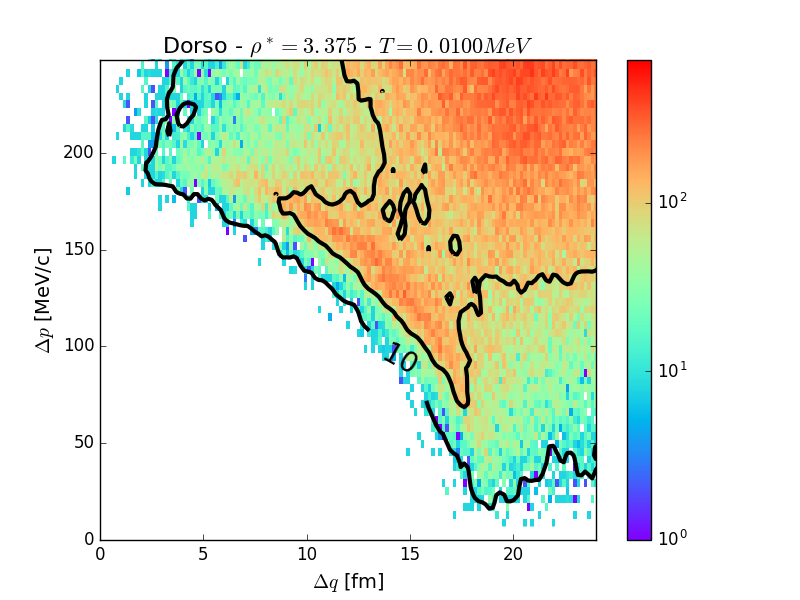
\includegraphics[trim = 5mm 0mm 50mm 5mm, clip, height=0.3\textwidth]{pauli_gas/exclusion/exclusion_zoom_rho0_dorso_0,01.png}
	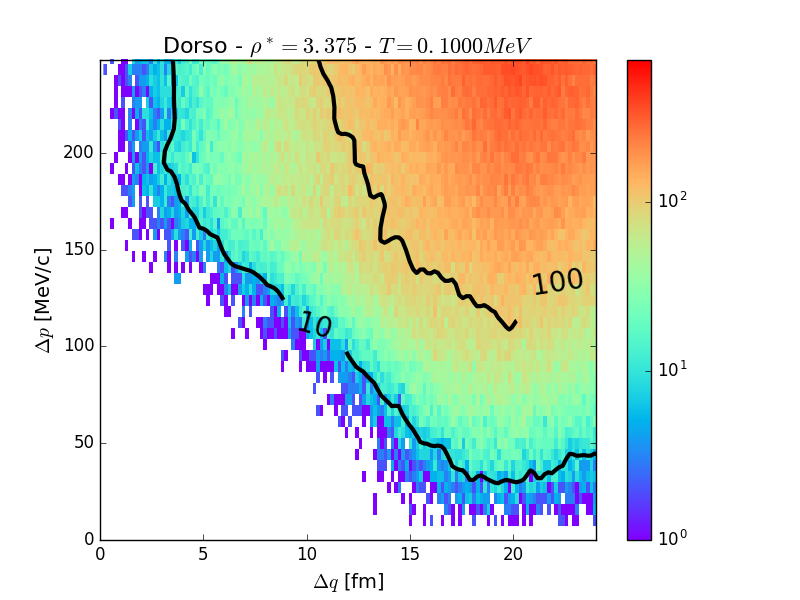
\includegraphics[trim = 24mm 0mm 50mm 5mm, clip, height=0.3\textwidth]{pauli_gas/exclusion/exclusion_zoom_rho0_dorso_0,1.png}
	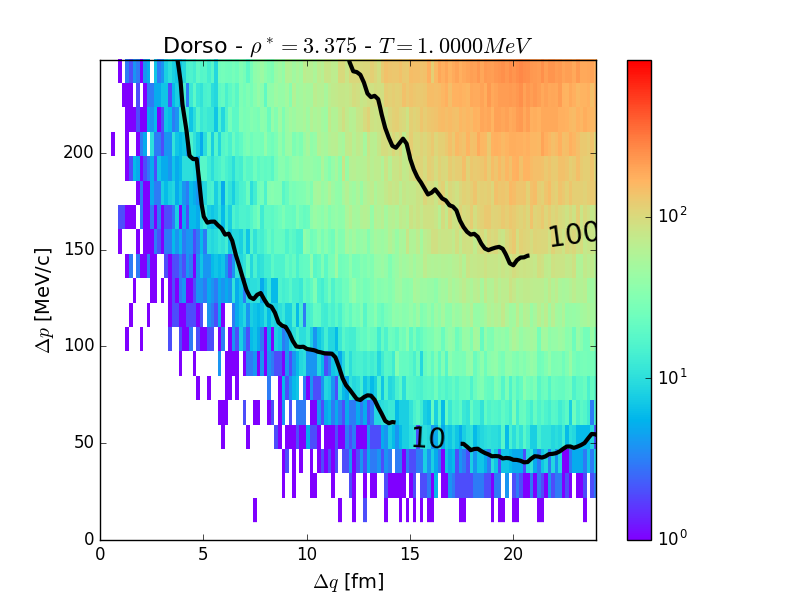
\includegraphics[trim = 24mm 0mm 20mm 5mm, clip, height=0.3\textwidth]{pauli_gas/exclusion/exclusion_zoom_rho0_dorso_1.png}
	\caption{Acercamiento a la región de interés cerca del origen. Se evidencia la aparición de una región excluida a medida que desciende $T$.}
	\label{fig:exclusion_zoom_rho0_dorso}
\end{figure}

Resulta entonces razonable cuestionarse si estos histogramas coinciden realmente con los de un gas ideal a $T$ suficientemente alta.
Las distribuciones de un gas ideal son conocidas, siendo las part\`iculas independientes; tienen distribución uniforme dentro de la caja en $\mathbf{q}$ y una
distribución de MB en su impulso según \eqref{eq:dist_MB_imp}.
Simulamos entonces 8 configuraciones distintas usando estas distribuciones y analizamos su espacio de $\Delta y$ como antes.
Para $T=3MeV$ y $\rho^*=3.375$ podemos apreciar los resultados para el gas ideal y para el potencial con parámetros de Dorso.
Estos gráficos resultan muy similares, mostrando la clara tendencia hacia el gas ideal para $T$ alta.

\begin{figure}[H]
	\centering	%trim={<left> <lower> <right> <upper>}
	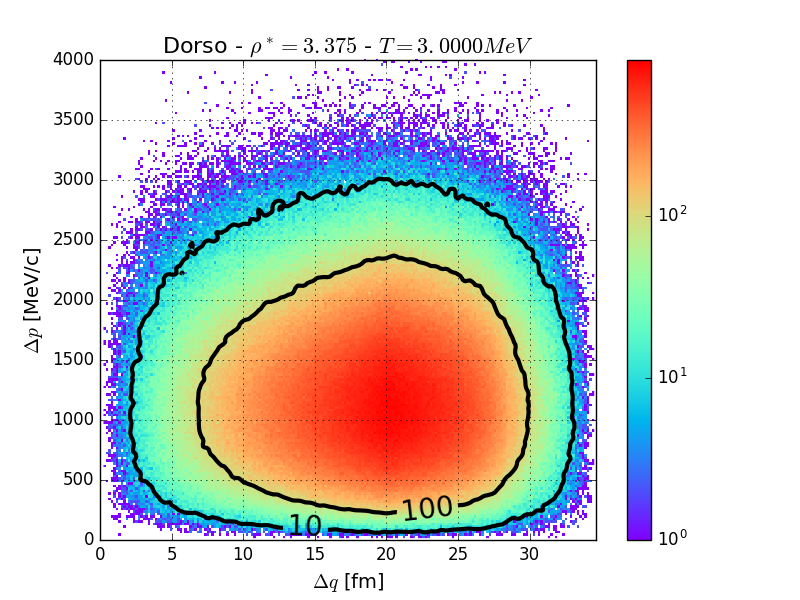
\includegraphics[trim = 5mm 0mm 50mm 5mm, clip, height=0.3\textwidth]{pauli_gas/exclusion/exclusion_rho0_dorso_3.png}
	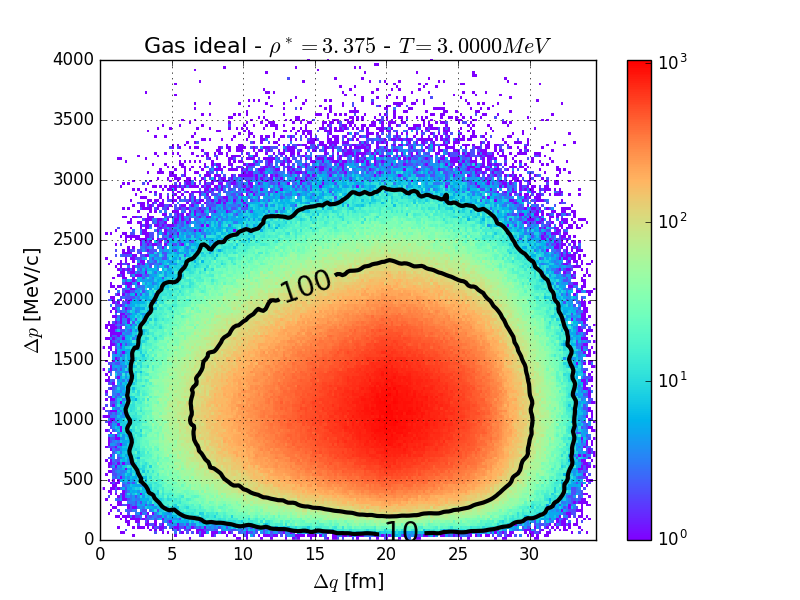
\includegraphics[trim = 24mm 0mm 20mm 5mm, clip, height=0.3\textwidth]{pauli_gas/exclusion/exclusion_rho0_GIvsdorso_3.png}
	\caption{Comparación de gas de Pauli con parámetros de Dorso y gas ideal.
  La coincidencia resulta evidente y muestra que siempre existe una región despoblada cerca del origen, pero no elíptica.}
	\label{fig:exclusion_dorso_vs_GI}
\end{figure}

Es interesante notar que tampoco para gas ideal clásico tenemos mucha población cerca del origen.
Esto ciertamente puede deberse a cuestiones estadísticas; la probabilidad de que 2 partículas se superpongan exactamente es nula y decrece como
$\sim\Delta q**2\Delta p**2$ para $\Delta y\to0$ gracias al jacobiano de esféricas.

Sabiendo que efectivamente existe un región excluida, la siguiente cuestión es analizar si es la misma que para el choque unidimensional.
Para esto podemos analizar el área que estudiamos previamente, en particular los resultados de $A^*$.
Conociendo el area de cada bin, podemos contar la cantidad que están desocupados en un entorno del origen y así estimar el área de la región excluida.
En la \textbf{Figura \ref{fig:AvsT}} podemos apreciar el área reducida $A^*$ en función de la temperatura para las distintas densidades y conjuntos de parámetros.
Además, marcamos el valor estimado para $A^*$ en la sección \ref{sec:choque1D} para el $D^*$ correspondiente a cada conjunto de parámetros.
El caso de Dorso es muy consistente con el resultado anterior, reduciéndose a media que aumenta $T$ según lo esperado.
Por otro lado, el caso de Maruyama tiene un $A^*(T)$ muy similar, convergiendo para $T$ baja al mismo valor de $A^*(D^*_D)\sim 26 \neq A^*(D^*_M)\sim 38$.
Es posible que no hayamos alcanzado temperaturas suficientemente bajas en el caso de Maruyama, razón por la cual el área excluida del histograma es menor a la real.

\begin{figure}[H]
	\centering	%trim={<left> <lower> <right> <upper>}
	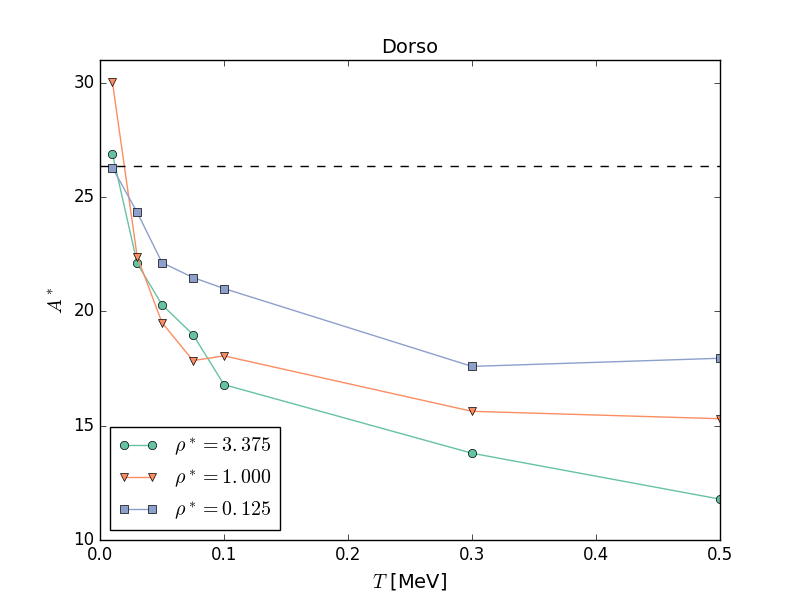
\includegraphics[trim = 5mm 0mm 10mm 5mm, clip, width=0.4\textwidth]{pauli_gas/AvsT_dorso.png}
	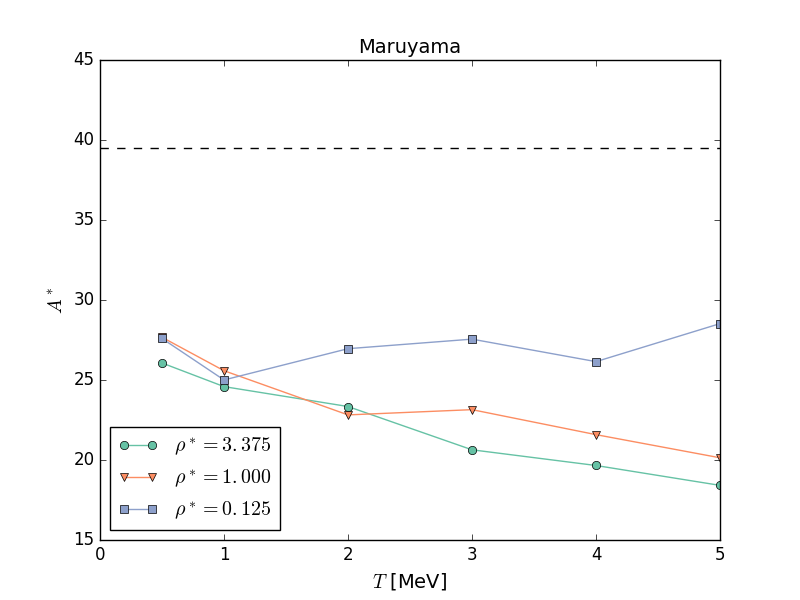
\includegraphics[trim = 5mm 0mm 10mm 5mm, clip, width=0.4\textwidth]{pauli_gas/AvsT_maruyama.png}
	\caption{Area reducida en función de temperatura obtenida de los histogramas 2D.
  La línea punteada marca el valor de $A^*$ para el $D^*$ de cada configuración, pero solo resulta coincidente para los parámetros de Dorso.}
	\label{fig:AvsT}
\end{figure}


\subsection{Distribución de energía cinética}{\label{sec:dist_energ}}

Con toda esa información, hicimos los histogramas de energía cinética del Pauli gas y los comparamos con las distribuciones de Fermi-Dirac (FD) y Maxwell-Boltzmann (MB)
a esa misma $T$ y $\rho$ y con la misma masa $m$, según las ecuaciones \eqref{eq:dist_FD} y \eqref{eq:dist_MB}, respectivamente.

\begin{figure}[H]
	\centering
	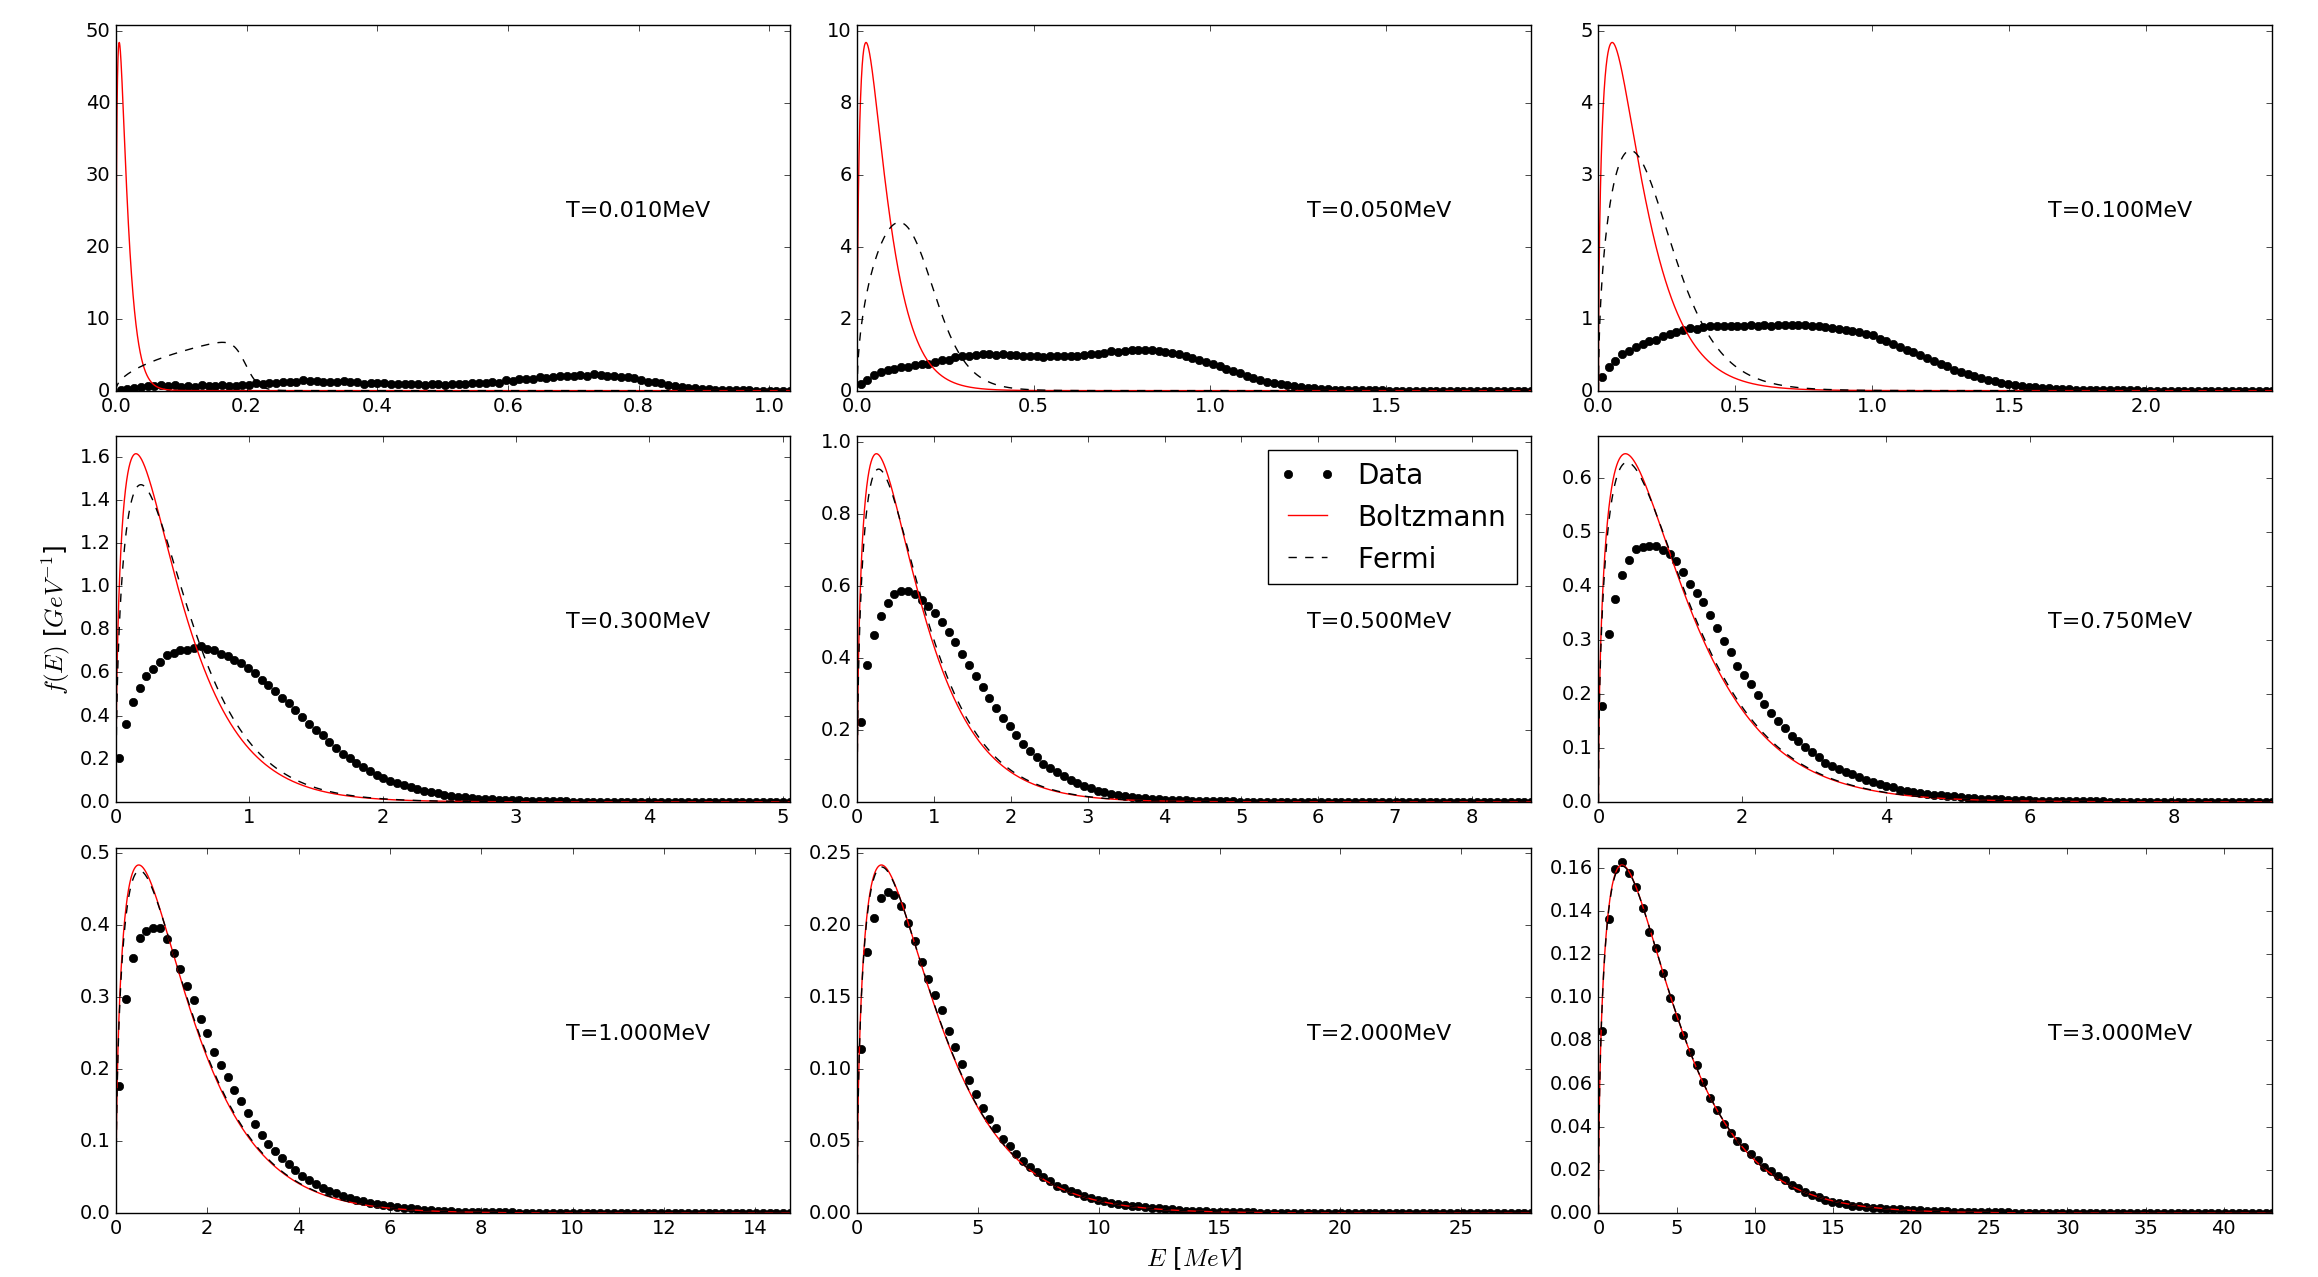
\includegraphics[width=0.9\textwidth]{pauli_gas/histogramas/hist_rho0_dorso.png}
	\caption{Distribuciones de energía cinética para los parámetros de Dorso en \eqref{eq:params_dorso} y $\rho^* = \rho_o^* = 3.375$}
	\label{fig:hist_rho0_dorso}
\end{figure}

\begin{figure}[H]
	\centering
	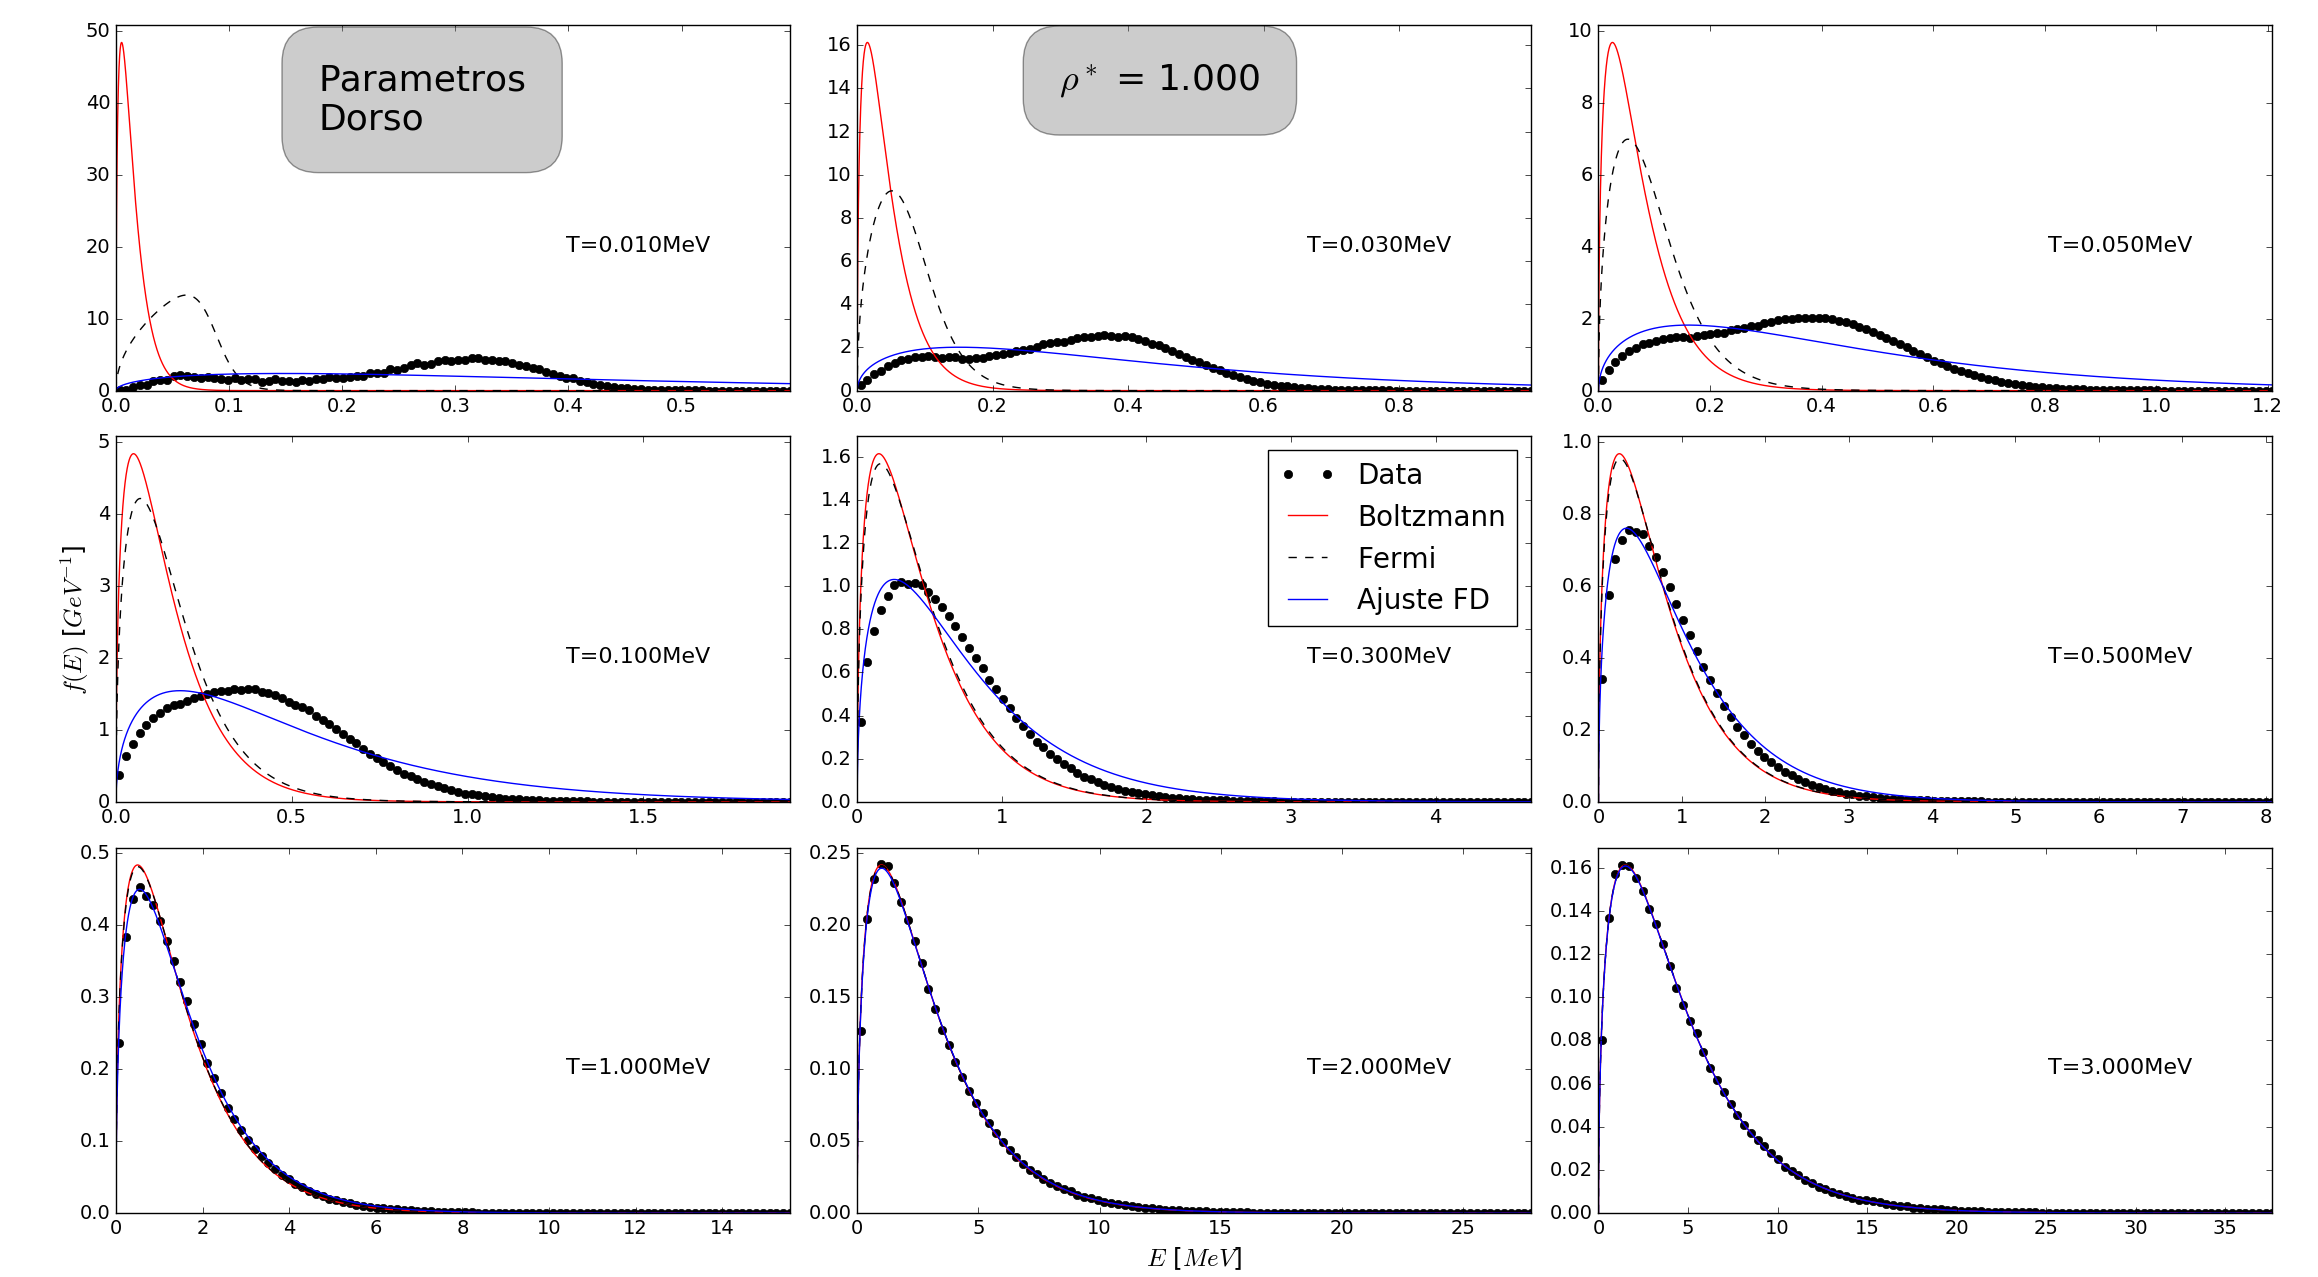
\includegraphics[width=0.9\textwidth]{pauli_gas/histogramas/hist_rho1_dorso.png}
	\caption{Distribuciones de energía cinética para los parámetros de Dorso en \eqref{eq:params_dorso} y $\rho^* = \rho_1^* = 1$}
	\label{fig:hist_rho1_dorso}
\end{figure}
\begin{figure}[H]
	\centering
	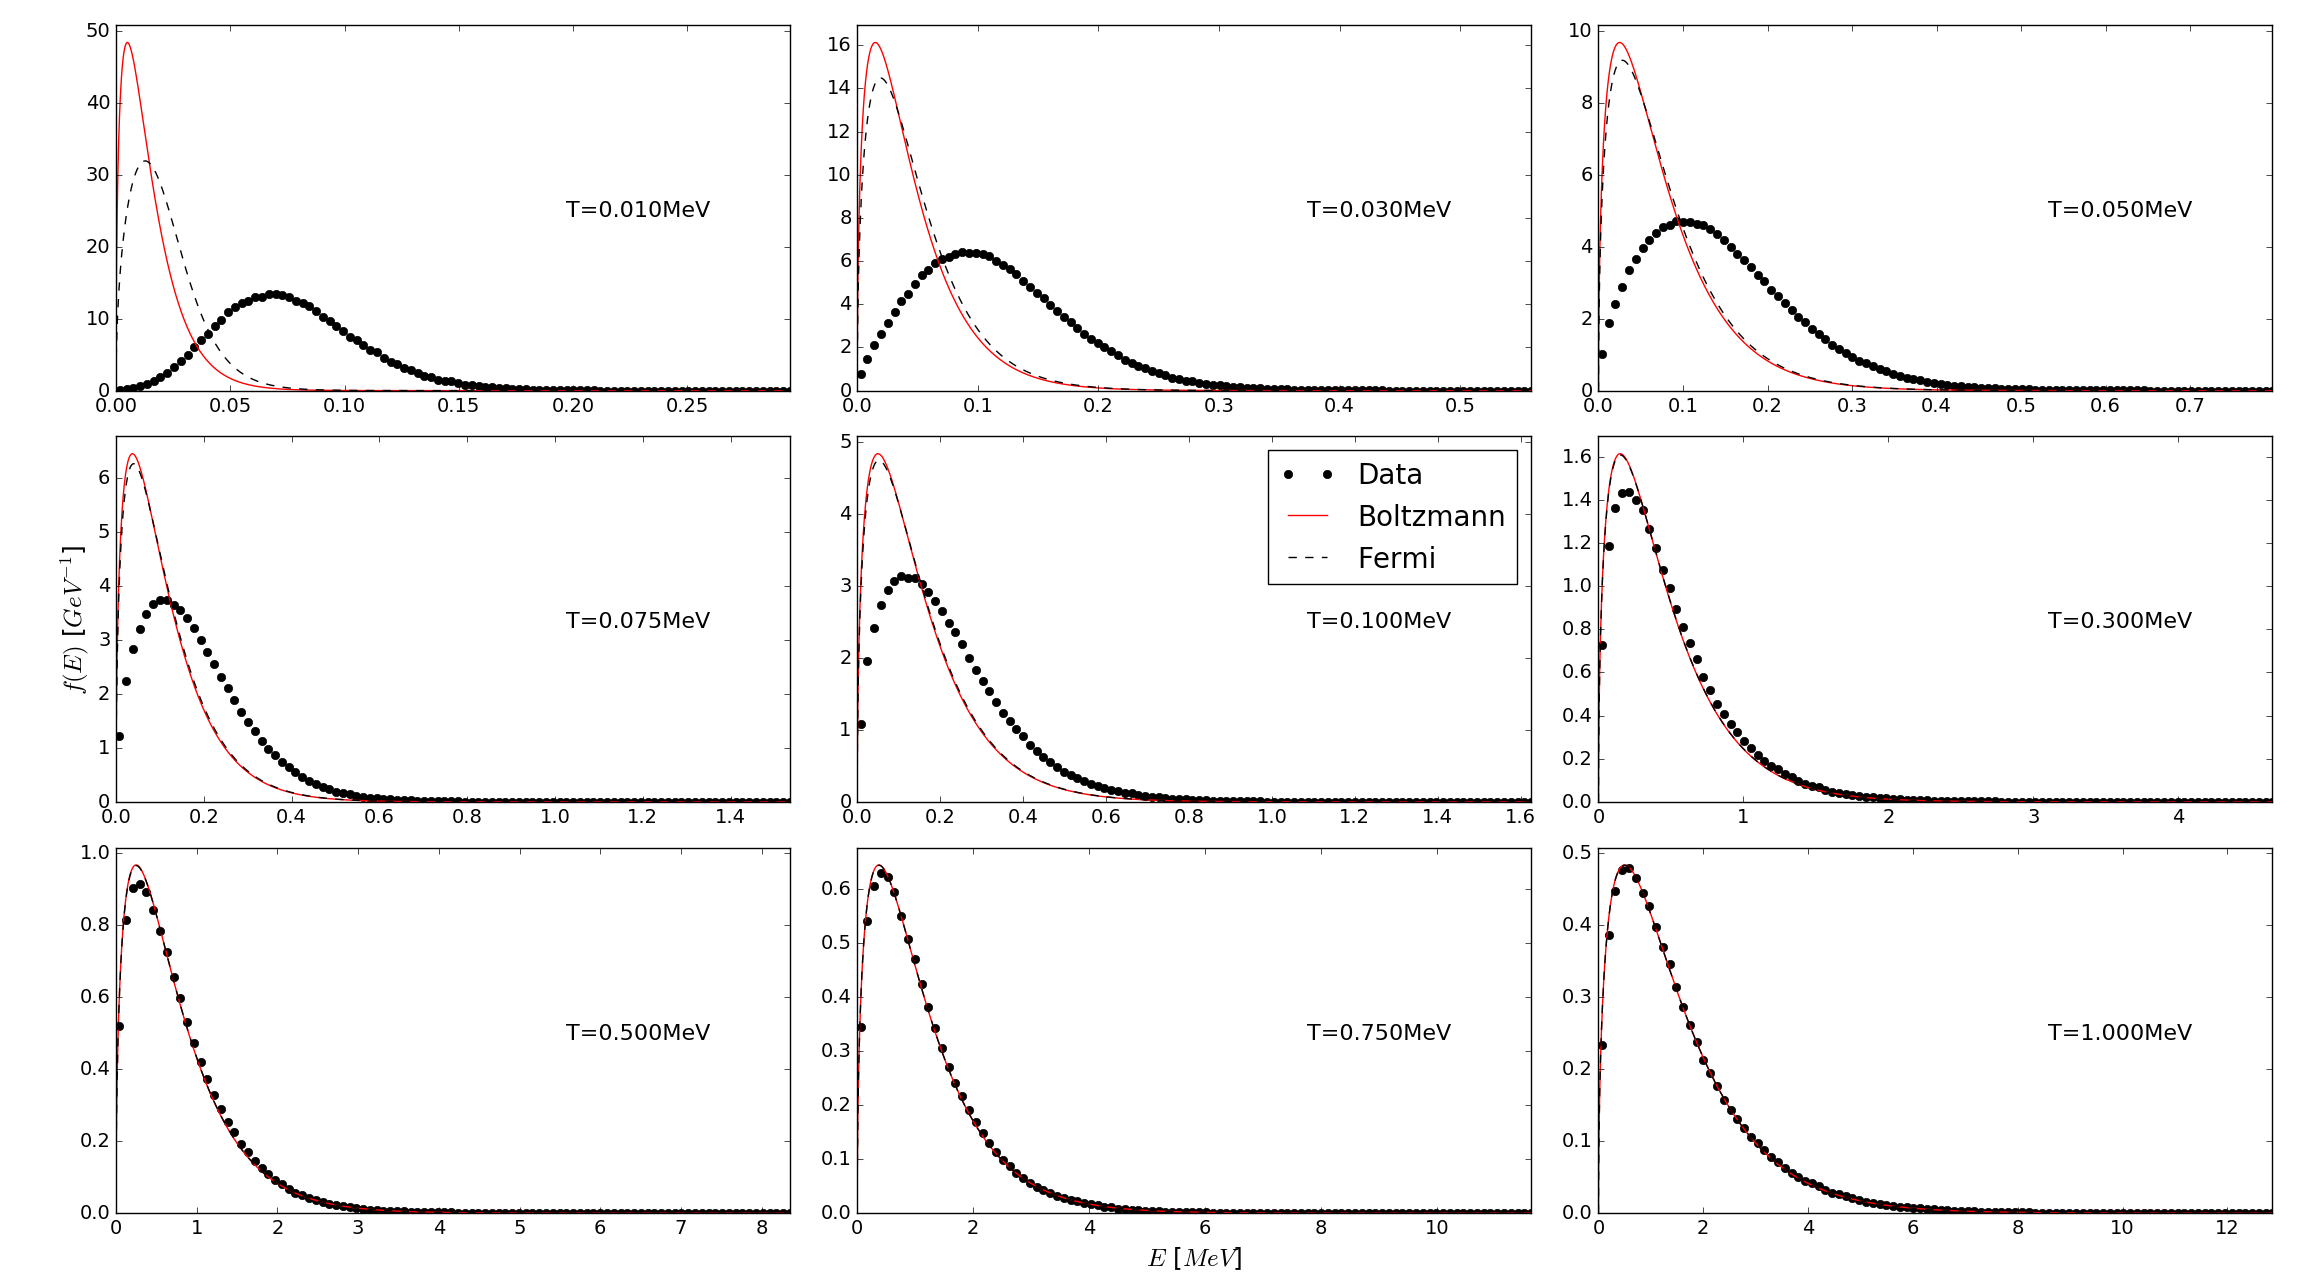
\includegraphics[width=0.9\textwidth]{pauli_gas/histogramas/hist_rho2_dorso.png}
	\caption{Distribuciones de energía cinética para los parámetros de Dorso en \eqref{eq:params_dorso} y $\rho^* = \rho_2^* = 0.125$}
	\label{fig:hist_rho2_dorso}
\end{figure}

Comenzando con los parámetros \eqref{eq:params_dorso}, vemos los histogramas de las 3 densidades en las \textbf{Figuras \ref{fig:hist_rho0_dorso}},
\textbf{\ref{fig:hist_rho1_dorso}} y \textbf{\ref{fig:hist_rho2_dorso}} para algunas temperaturas seleccionadas.
Además de compararlos con las distribuciones de MB y FD, incluimos un ajuste por la distribución de FD \eqref{eq:dist_FD} pero dejando $T$ y $\mu$ como parámetros libres del ajuste.
Esto último equivale a buscar los $T'$ y $\rho'$ cuya distribución de FD es más similar a la distribución de Pauli; es considerar que es posible que nuestro gas de Pauli
emule un gas de Fermi bajo distintas condiciones termodinámicas.

En los 3 casos, podemos apreciar como la distribución se aleja de MB a medida que la temperatura desciende según lo esperado.
Sin embargo, esta separación comienza a una temperatura mayor que la separación de FD respecto a MB.
De hecho, los datos no tienden a acercarse a FD luego de alejarse de MB; solo hay coindicencia de las 3 distribuciones (simultaneamente) a $T$ alta.
Similar a FD, el pico del histograma de los datos no parece acercarse al origen, una de las principales diferencias con MB.
Sin embargo, este pico se da para energías cinéticas mucho mayores que el de FD, lo cual hace pensar que este gas de Pauli sobreestima la exclusión entre las particulas, alejándolas
más de lo que debería.

Más particularmente, podemos notar que la distribución a $T$ baja para $\rho_o^*$ y $\rho_1^*$ tiene 2 máximos en lugar de uno, lo cual es muy llamativo.
Para $\rho_2^*$, solo hay un máximo, pero la curva entre este máximo y el origen es cóncava en lugar de convexa a diferencia tanto de MB como FD como de las otras densidades.
Además, la separación de los datos respecto a MB se da a temperaturas cada vez menores a medida que aumentamos $\rho^*$, lo cual también ocurre con FD.
Esto es razonable, dado que la noción de temperatura alta está muy asociada a la de densidad baja como discutimos en \ref{sec:intro_fermi_gas}.

Por el lado de los ajustes, los resultados son prometedores principalmente para temperaturas intermedias; temperaturas para las cuales FD y MB aún no difieren demasiado.
Esto nuevamente depende de $\rho$, pues los ajustes son razonablemente acertados para $T\geq 0.5MeV$ en el caso $\rho^*=3.375$, $T\geq 0.3MeV$ para $\rho^*=1$ y $T\geq 0.1MeV$ para $\rho^*=0.125$.

Con los histogramas obtenidos utilizando los parámetros de Maruyama \eqref{eq:params_maruyama} ocurre algo muy similar, como puede verse en las \textbf{Figuras \ref{fig:hist_rho0_maruyama}},
\textbf{\ref{fig:hist_rho1_maruyama}} y \textbf{\ref{fig:hist_rho2_maruyama}}.
Sin embargo, es ciertamente notable que la forma del histograma de los datos parece acompañar mejor a la distribución de FD y que los ajustes por FD resultan mucho más certeros, siendo
razonables para valores de $T$ considerablemente bajos.
Además, surge inmediatamente la diferencia de escalas entre temperaturas; las transiciones de las distribuciones del Pauli gas ocurren a $T$ un orden de magnitud mayor para estos parámetros.
Esto es llamativo y puede ciertamente estar asociado al hecho de que el $D^*$ mismo aumentó un orden de magnitud.

Esto ocurre en menor medida para la distribución de FD.
Es razonable que ocurra dado que, aunque los $\rho^*$ no cambiaron, si lo hicieron las densidades $\rho$ al cambiar el $q_o$.
Dado que el $q_o$ de Maruyama es menor, las densidades $\rho$ aumentaron, redefiniendo la noción de alta temperatura para valores de $T$ mayores.
Esto ciertamente nos muestra que el parámetro $q_o$ también influye a la hora de simular una distribución de FD vía un gas de Pauli.
\begin{figure}[H]
	\centering
	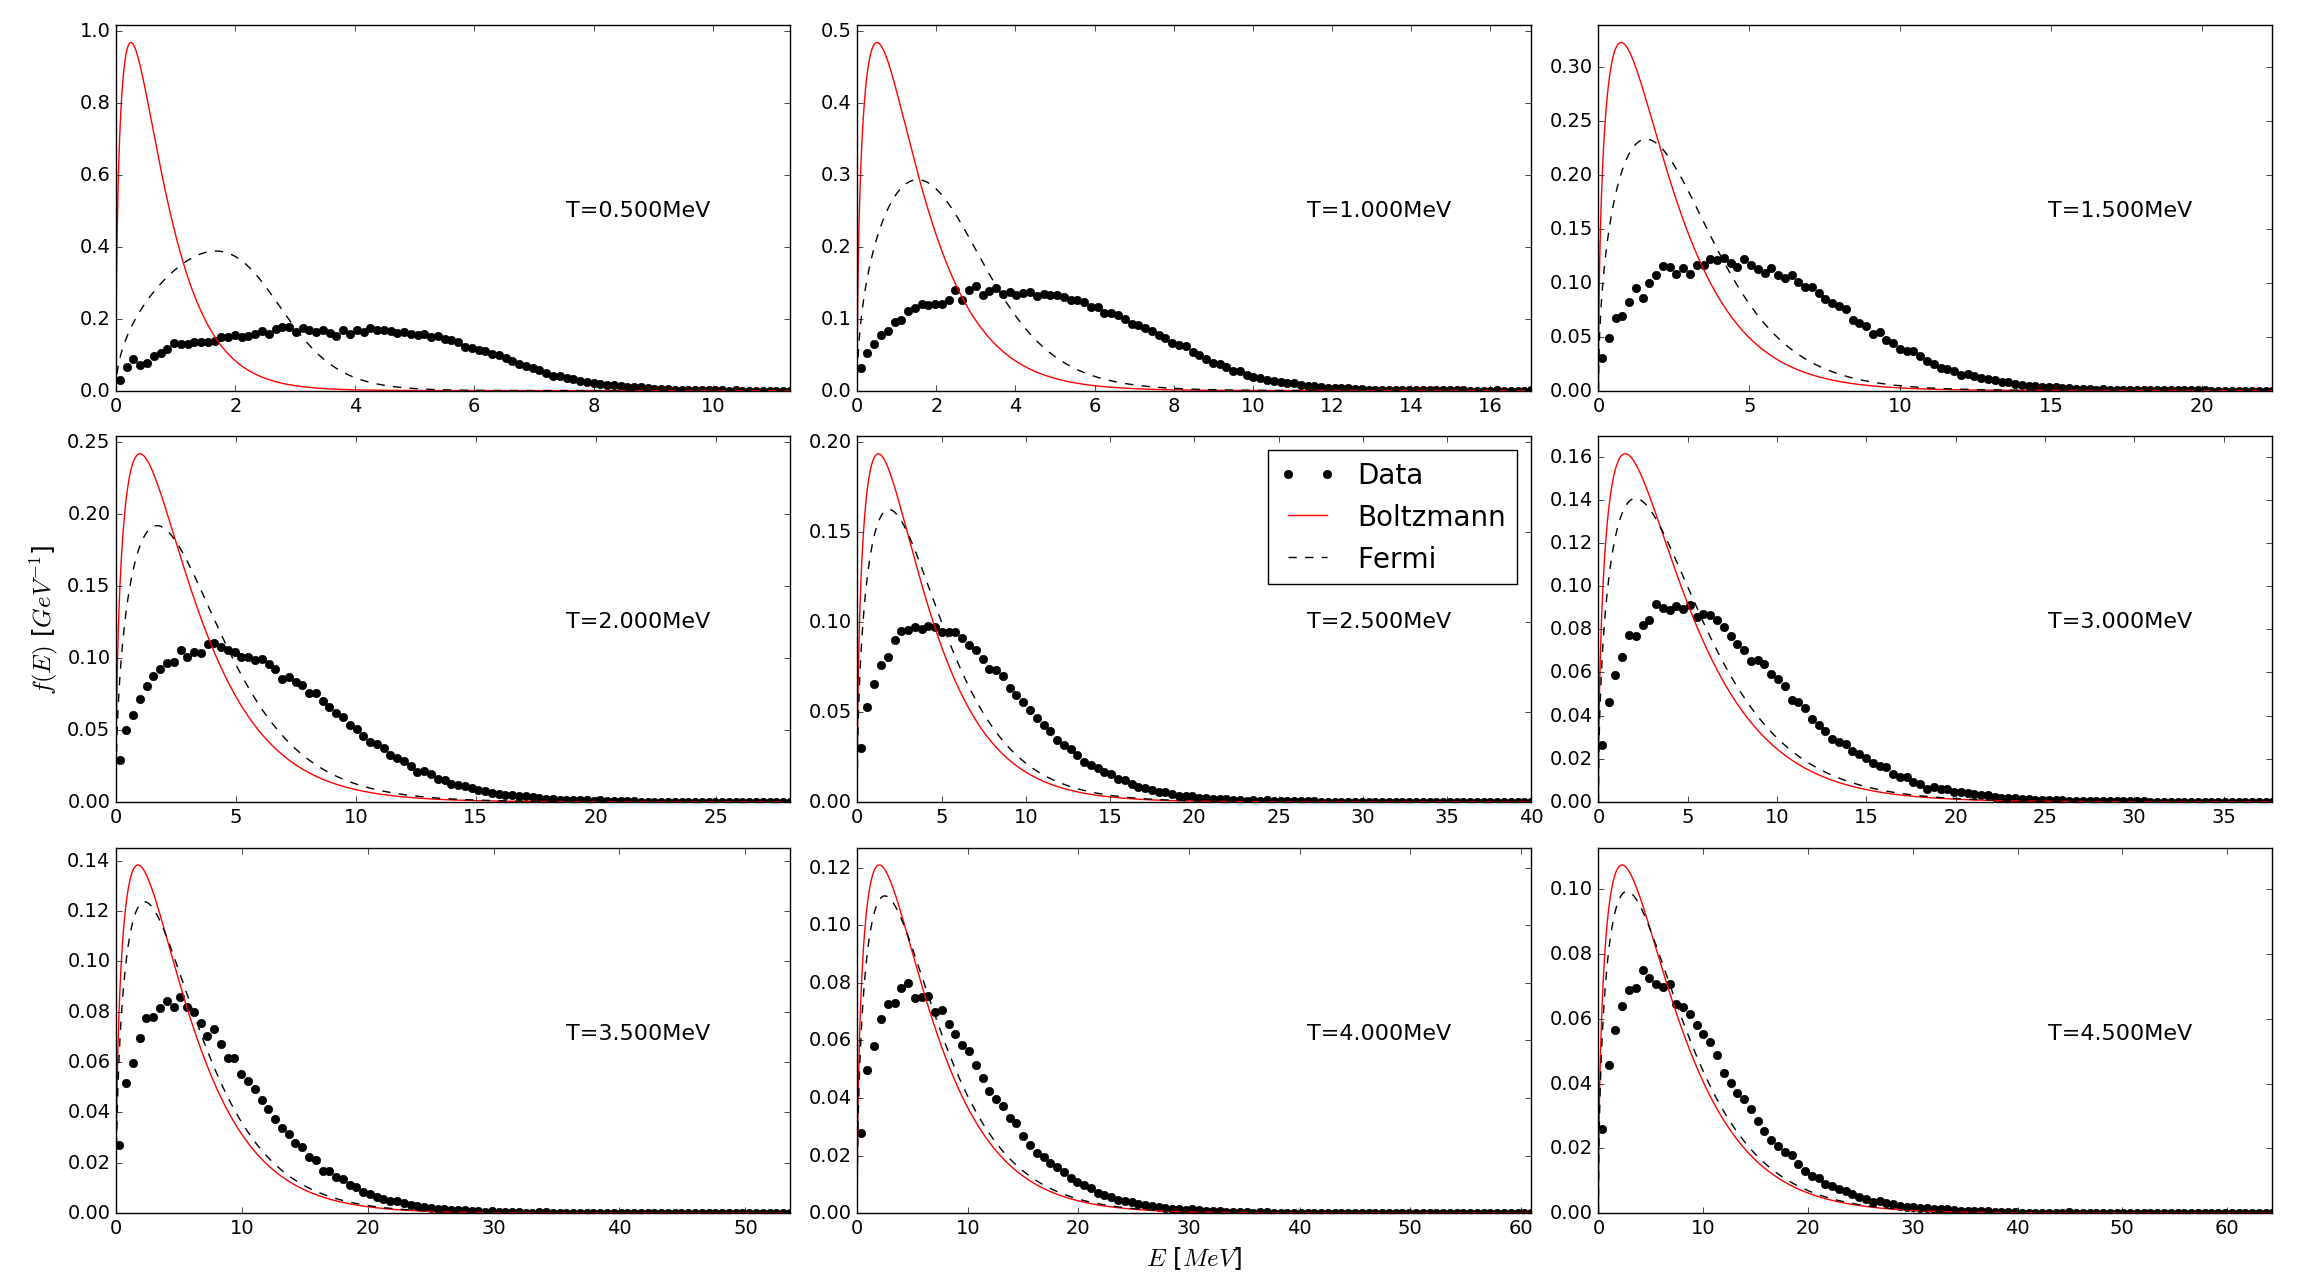
\includegraphics[width=0.9\textwidth]{pauli_gas/histogramas/hist_rho0_maruyama.png}
	\caption{Distribuciones de energía cinética para los parámetros de Maruyama en \eqref{eq:params_maruyama} y $\rho^* = \rho_o^* = 3.375$}
	\label{fig:hist_rho0_maruyama}
\end{figure}
\begin{figure}[H]
	\centering
	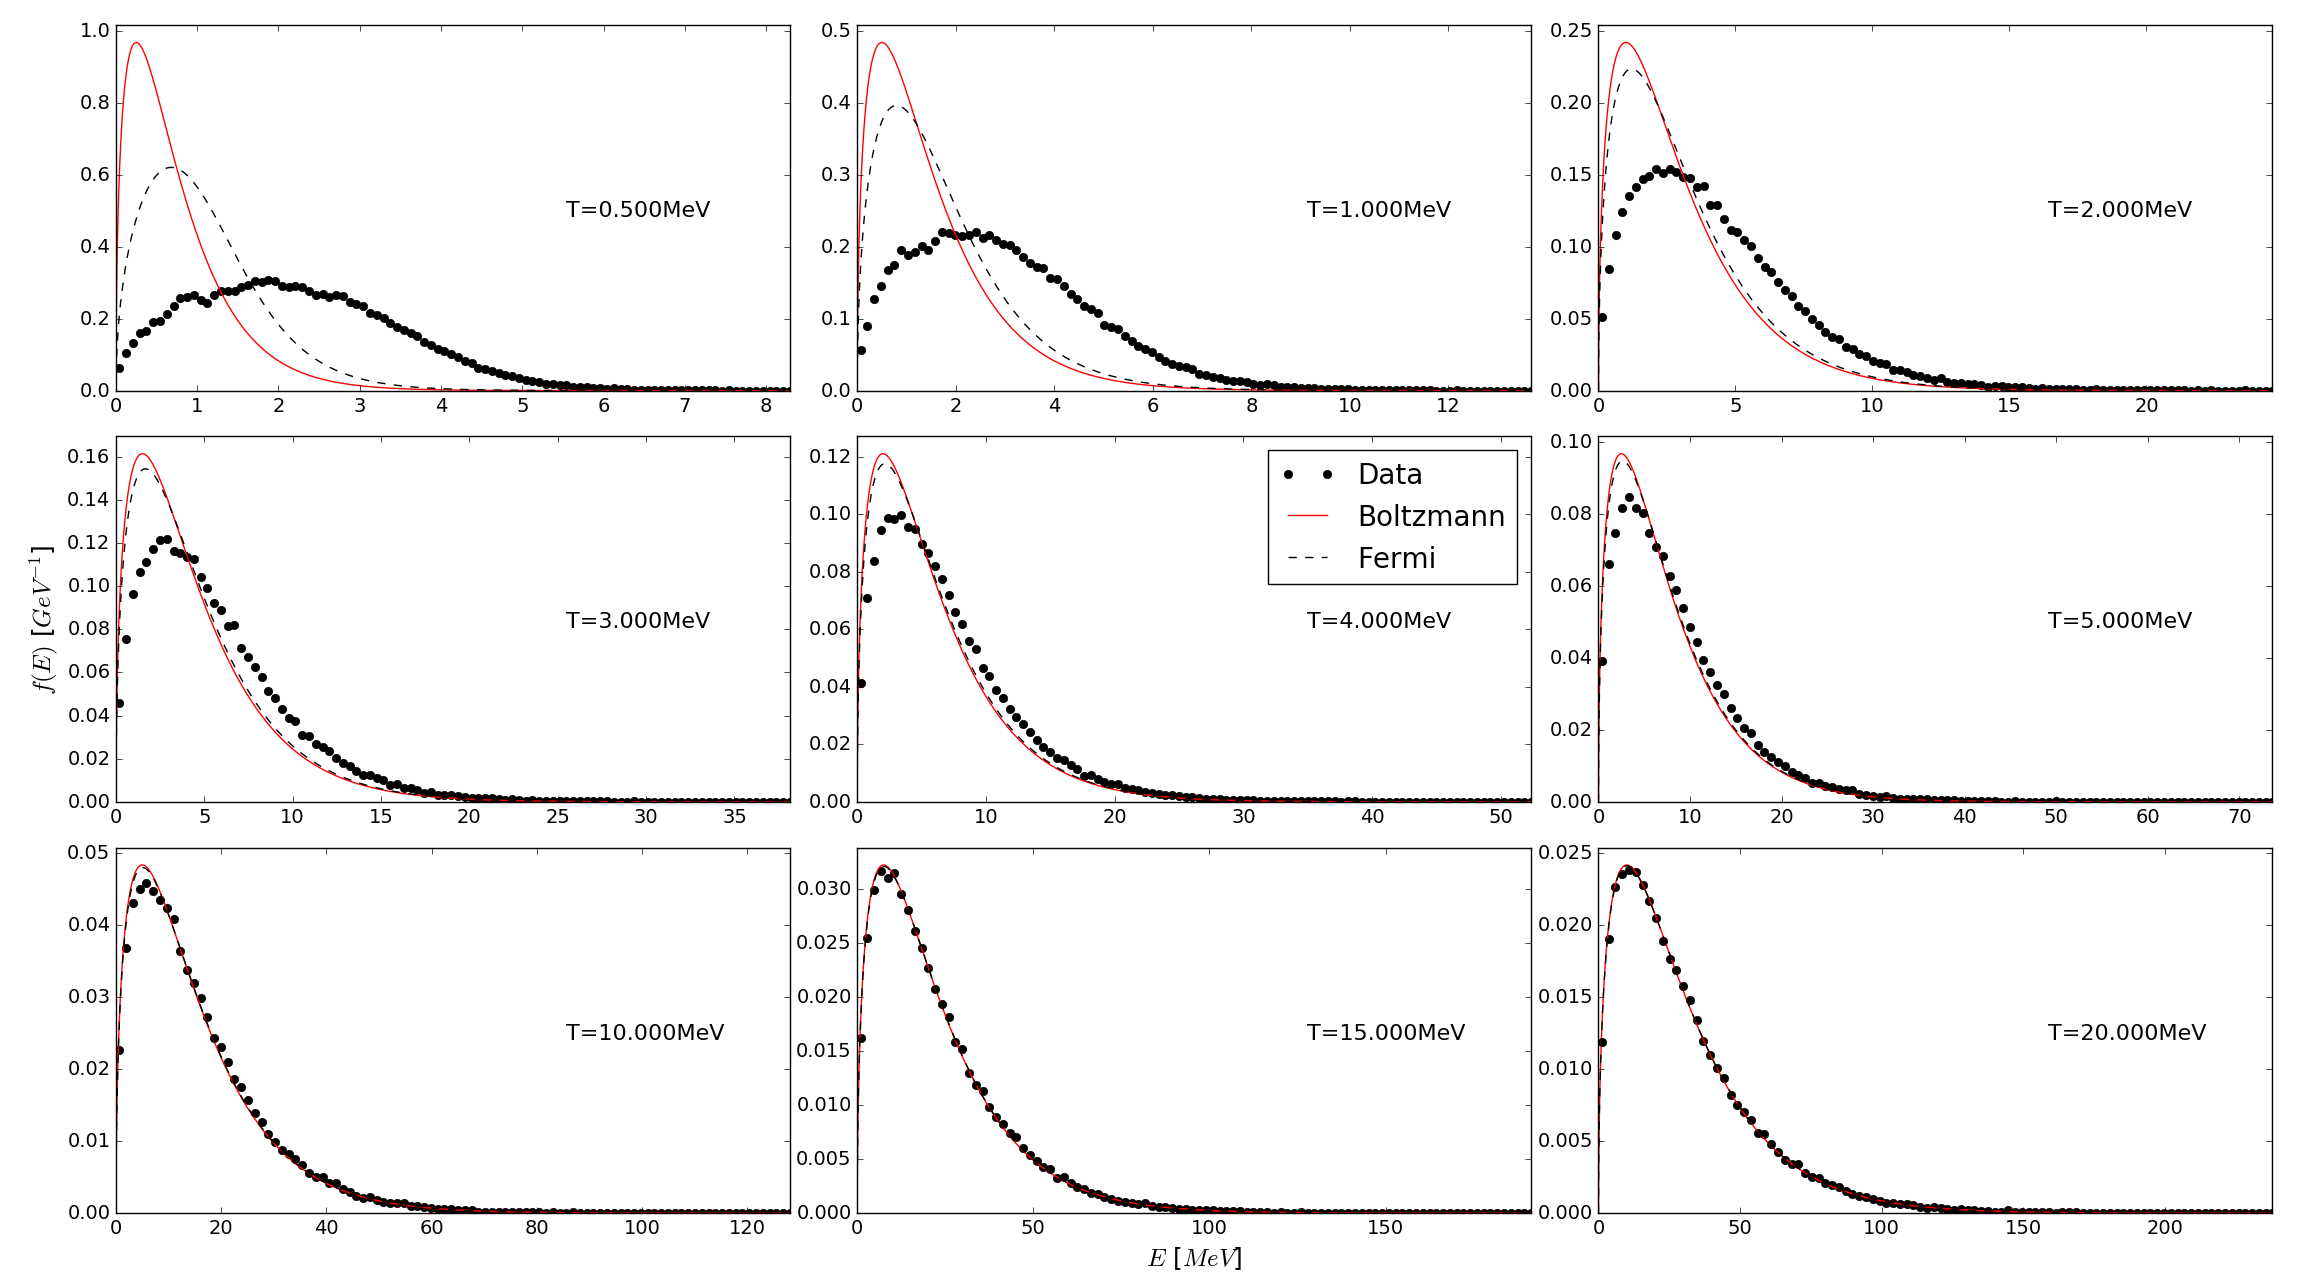
\includegraphics[width=0.9\textwidth]{pauli_gas/histogramas/hist_rho1_maruyama.png}
	\caption{Distribuciones de energía cinética para los parámetros de Maruyama en \eqref{eq:params_maruyama} y $\rho^* = \rho_1^* = 1$}
	\label{fig:hist_rho1_maruyama}
\end{figure}
\begin{figure}[H]
	\centering
	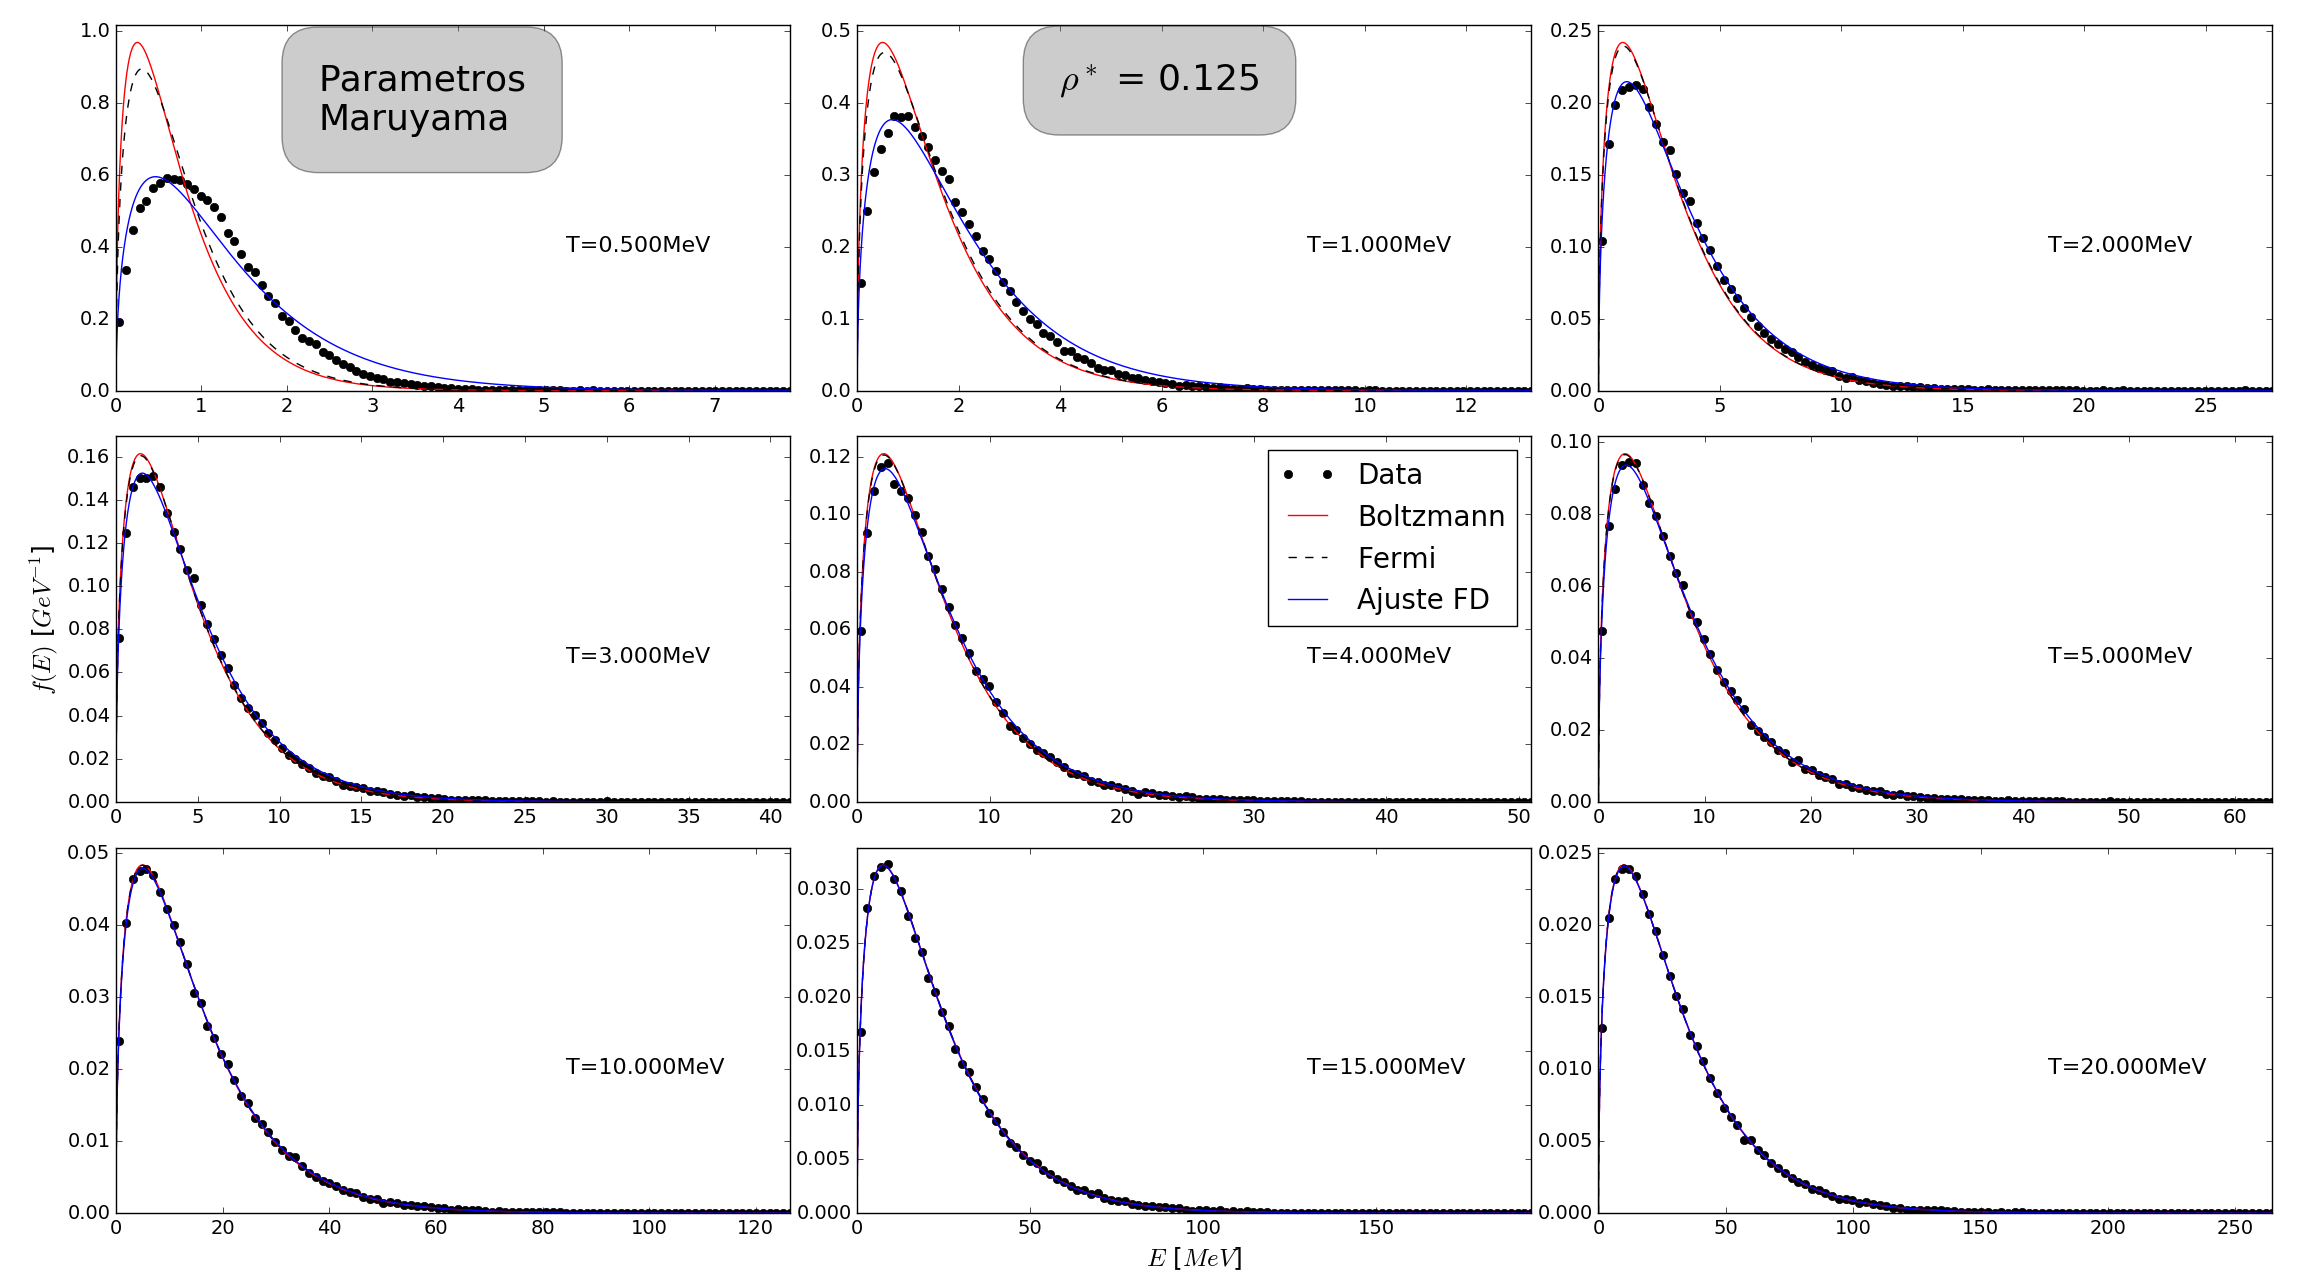
\includegraphics[width=0.9\textwidth]{pauli_gas/histogramas/hist_rho2_maruyama.png}
	\caption{Distribuciones de energía cinética para los parámetros de Maruyama en \eqref{eq:params_maruyama} y $\rho^* = \rho_2^* = 0.125$}
	\label{fig:hist_rho2_maruyama}
\end{figure}

Los gráficos de las \textbf{Figuras \ref{fig:muvsT}} y \textbf{\ref{fig:TvsT}} muestran la dependencia de los parámetros ajustados con la temperatura
$T$ y la densidad reducida $\rho^*$ para ambos conjuntos de parámetros.
Podemos ver que tanto para los parámetros de Dorso como para los de Maruyama, el comportamiento cualitativo es el mismo.
Para empezar, los gráficos de la \textbf{Figura \ref{fig:muvsT_dorso}} y \textbf{Figura \ref{fig:muvsT_maruyama}} muestran que el $\mu$ de FD tiende a la energía de Fermi $E_F\equiv \mu(T=0,\rho)$,
confirmado que en todos los casos alcanzamos el régimen de bajas temperaturas para FD.
Notamos además que para $T$ alta, ambos $\mu$ coinciden, lo cual es razonable dado que estamos en MB, pero a medida que $T$ desciende vemos que $\mu_{aj}\leq\mu_{FD}$.
A pesar de que la coincidencia para $\rho^*=3.375$ es practicamente inexistente, para $\rho^*=0.125$ esta coincidencia se da en todo el rango de $T$ estudiado.
Algo muy similar ocurre para la $T_{aj}$, que resulta siempre levemente superior a $T$.
Es justamente este $T_{aj}$ quien marca la diferencia entre el ajuste por FD y el FD exacto para $\rho^*=0.125$ donde $\mu_{aj}\approx\mu_{FD}$.

Estas propiedades marcan los dos defectos de Pauli respecto a FD; $T_{aj}\geq T$ implica que la cola de la distribución se extiende para $E$ mayores mientras que $\mu_{aj}\leq\mu_{FD}$ tiende a
desplazar el máximo de la distribución a $E$ mayores.

\begin{figure}[H]
	\centering
	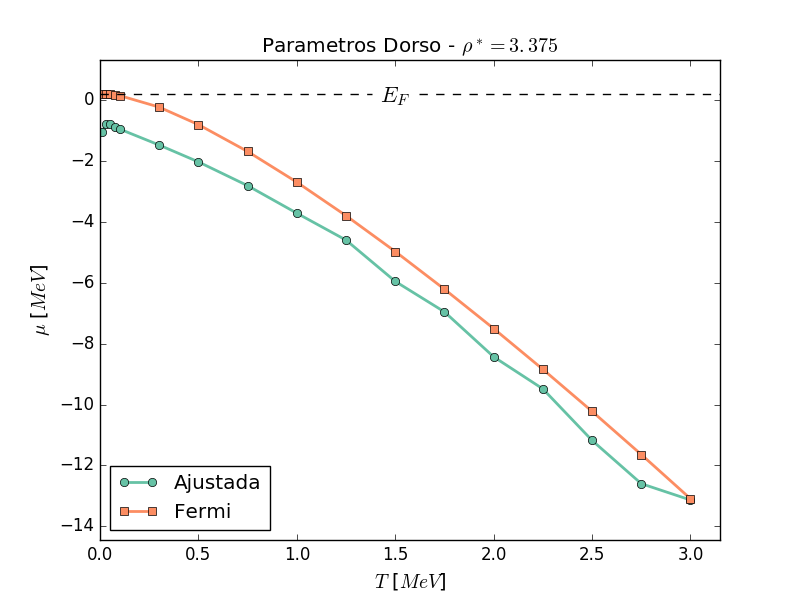
\includegraphics[trim = 5mm 0mm 20mm 5mm, clip, width=0.32\textwidth]{pauli_gas/muvsT_rho0_dorso.png}
	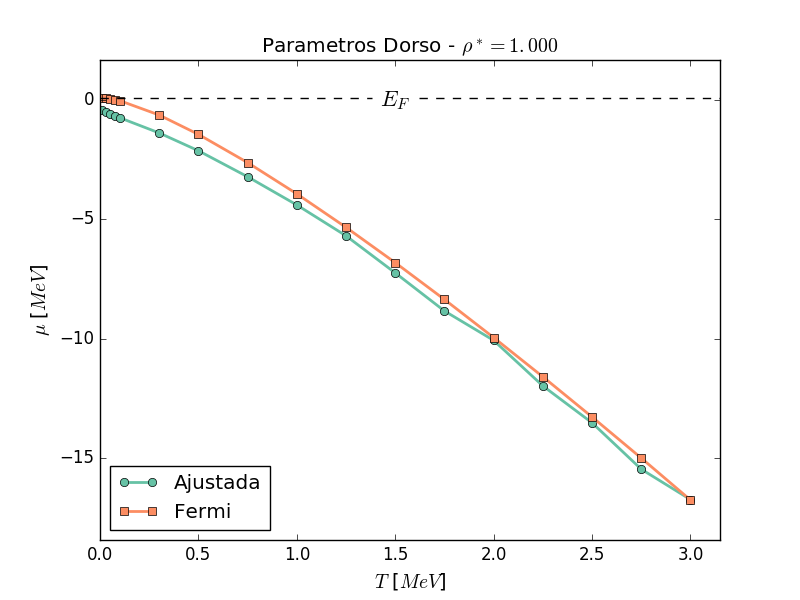
\includegraphics[trim = 5mm 0mm 20mm 5mm, clip, width=0.32\textwidth]{pauli_gas/muvsT_rho1_dorso.png}
	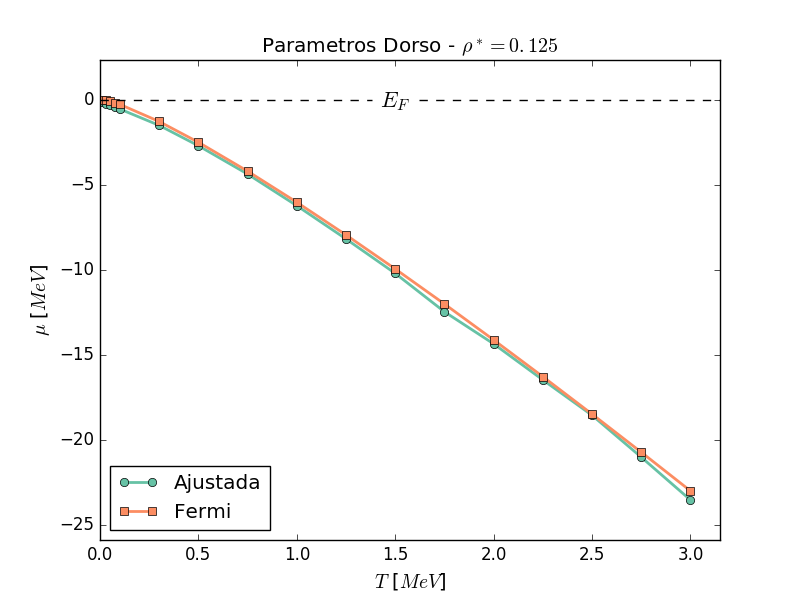
\includegraphics[trim = 5mm 0mm 20mm 5mm, clip, width=0.32\textwidth]{pauli_gas/muvsT_rho2_dorso.png}
	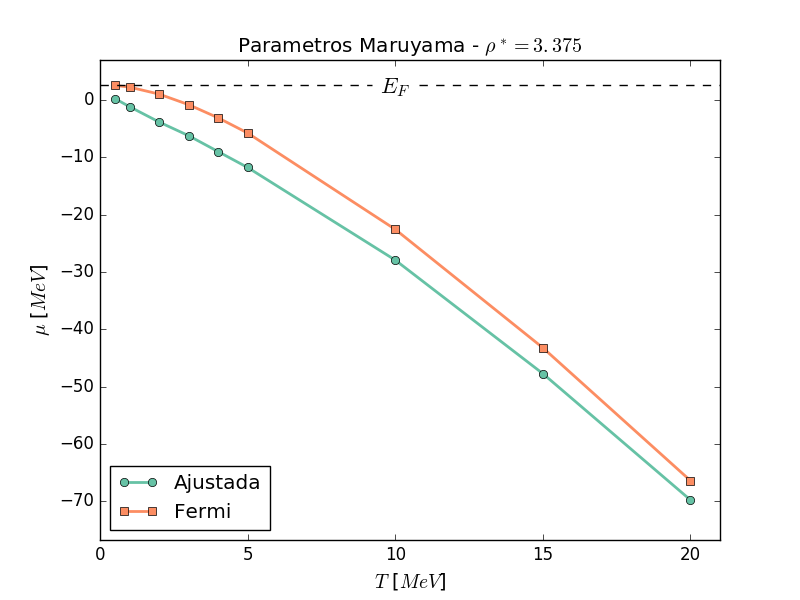
\includegraphics[trim = 5mm 0mm 20mm 5mm, clip, width=0.32\textwidth]{pauli_gas/muvsT_rho0_maruyama.png}
	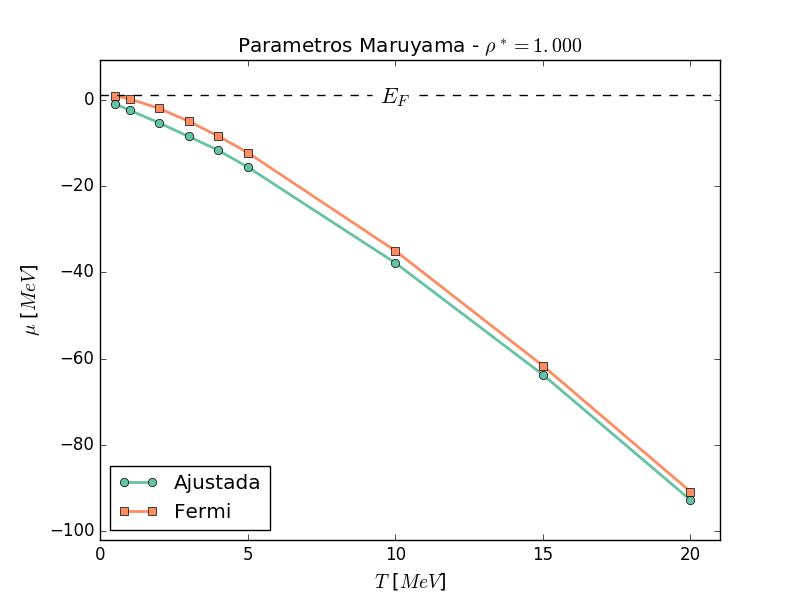
\includegraphics[trim = 5mm 0mm 20mm 5mm, clip, width=0.32\textwidth]{pauli_gas/muvsT_rho1_maruyama.png}
	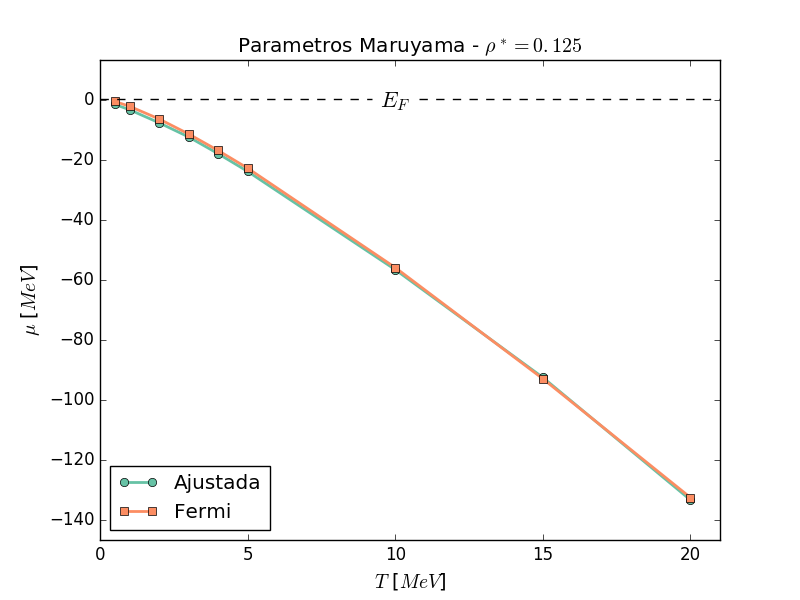
\includegraphics[trim = 5mm 0mm 20mm 5mm, clip, width=0.32\textwidth]{pauli_gas/muvsT_rho2_maruyama.png}
	\caption{Potencial químico exacto (FD) y el obtenido del ajuste en función de la temperatura del sistema.
  Ambos conjuntos de parámetros arrojan curvas cualitativamente similares, acercandose para $T$ mayores pero manteniendo $\mu_{aj}\leq \mu_{FD}$.}
	\label{fig:muvsT}
\end{figure}
\begin{figure}[H]
	\centering
	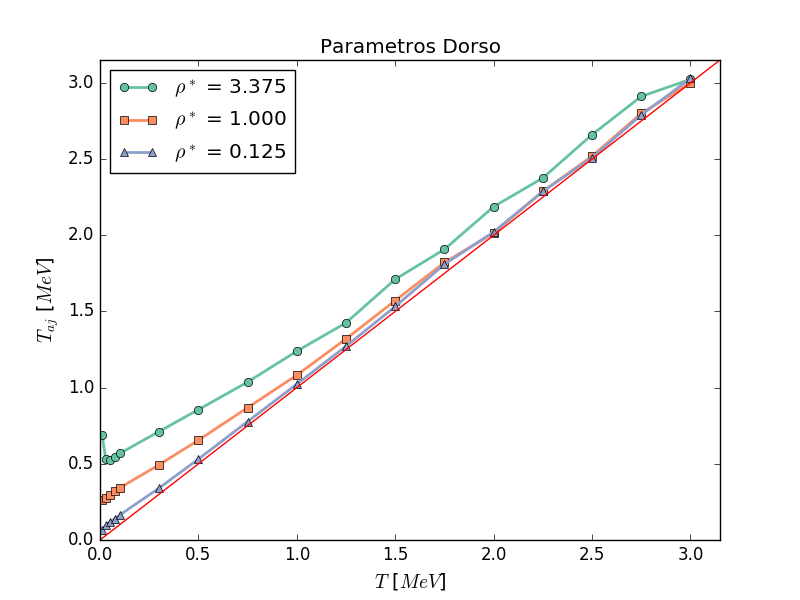
\includegraphics[trim = 5mm 0mm 20mm 5mm, clip, width=0.48\textwidth]{pauli_gas/TvsT_dorso.png}
	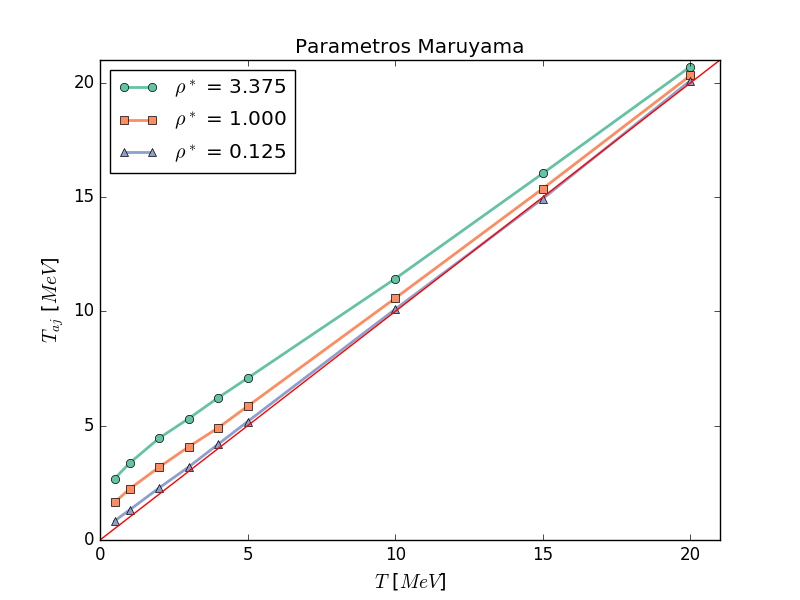
\includegraphics[trim = 5mm 0mm 20mm 5mm, clip, width=0.48\textwidth]{pauli_gas/TvsT_maruyama.png}
	\caption{Temperatura obtenida del ajuste en función de la temperatura del sistema para las 3 densidades reducidas estudiadas.
  La recta continua marca la identidad, a la que $T_{aj}$ tiende para alta $T$ para ambos conjuntos de parámetros.
  En general, es $T_{aj}\geq T$.}
	\label{fig:TvsT}
\end{figure}

Adicionalmente, podemos utilizar estos valores $T_{aj}$ y $\mu_{aj}$ para calcular la $\rho_{aj}$ correspondiente usando \eqref{eq:N_cont}, para analizar como estima el ajuste la densidad del sistema.
En la \textbf{Figura \ref{}} podemos apreciar que esta $\rho_{aj}$ resulta una clara sobreestimación de $\rho$, pero que cumple $\rho_{aj}\approx\rho$ para $T$ suficientemente grande.

\begin{figure}[H]
	\centering
	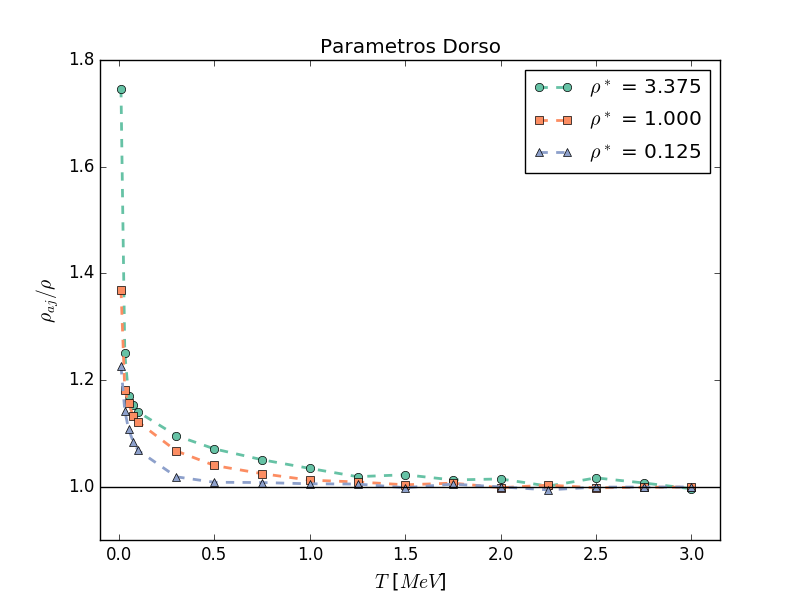
\includegraphics[trim = 5mm 0mm 20mm 5mm, clip, width=0.48\textwidth]{pauli_gas/rho_vs_T_dorso.png}
	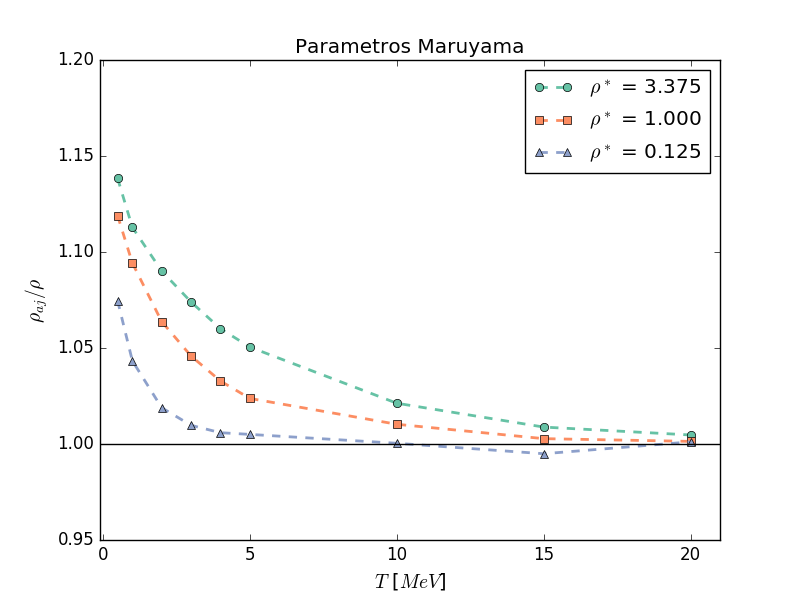
\includegraphics[trim = 5mm 0mm 20mm 5mm, clip, width=0.48\textwidth]{pauli_gas/rho_vs_T_maruyama.png}
	\caption{}
	\label{fig:rhovsT}
\end{figure}

Respecto a las diferencias, además de la ya discutida temperatura, el potencial químico $\mu$ resulta $\sim 6$ veces mayor respecto al obtenido por los parámetros de Dorso, nuevamente
debido a la diferencia en los $\rho$ introducida por el cambio de $q_o$.
Además, resulta interesante recalcar que aunque los ajustes por FD para Maruyama resultan mejores que los de Dorso, la calidad de las estimaciones $\mu_{aj}$ y $T_{aj}$
(respecto al $\mu$ y $T$ originales) es la misma.
Aún así, para Maruyama la sobreestimación de $\rho$ por $\rho_{aj}$ es menor al $15\%$ para todas las densidades, mientras que en el caso de Dorso llega hasta casi un $80\%$.
Por lo tanto, vemos que los parámetros de Maruyama generan una distribución más similar a un Fermi gas, pero no necesariamente al Fermi gas con la $T$ y $\rho$ del sistema.

%%%%%%%%%%%%%%%%%%%%%%%%%%%%%%%%%%%%%%%%%%%%%%%%%%%%%%%%%%%%%%%%%%%%%%%%%%%%%%%%%%%%%%%%%%%%%%%%%%%%%%%%%%%%%%%%%%%%%%%%%%%%%%%%%%%%%%%%%%%%%%%%%%%%%%%%%%%%%%%%%%%%%%%%%%%%%%%%%%%%%%%%%%%%%

Para entender esto, podemos nuevamente adimensionalizar el problema, analizando los parámetros que definen la forma de las distintas distribuciones.
Dado que las distribuciones de energía cinética $f(\varepsilon)$ son extensivas, podemos obtener una magnitud intensiva del sistema dividiendolas por el número de partículas $N$.
Esta nueva distribución intensiva solo puede depender de parámetros intensivos del sistema, como son la temperatura $T$ y la densidad $\rho$ pero también de parámetros microscópicos como
la masa $m$ y la constante de Planck $\hbar$.
Recordando las expresiones de $f_{FD}(\varepsilon)$ y $f_{MB}(\varepsilon)$ de \eqref{eq:dist_FD} y \eqref{eq:dist_MB}, vemos inmediatamente que podemos reescribir
\[ f_{MB}(\varepsilon;N,T) = \frac{N}{T}g_{MB}(\varepsilon^*) \]
\[ f_{FD}(\varepsilon;N, V, T, m, \hbar) = \frac{N}{T}g_{FD}(\varepsilon^*;\lambda^3\rho) \to \frac{N}{T}g_{MB}(\varepsilon^*) \text{ para } \lambda^3\rho\to0 \]
donde $\varepsilon^* = \varepsilon/T$ y $\lambda$ es la longitud de onda términa previamente definida.
En resumen, la adimensionalización nos permite eliminar 3 variables, mientras que la linealidad en $N$ nos permite eliminar una cuarta.

Podemos hacer un razonamiento análogo para la distribución $f_P(\varepsilon)$ de un gas de Pauli.
Los parámetros relevantes siguen siendo $T$, $\rho$ y $m$ pero también se suman los $D$, $q_o$ y $p_o$ del potencial de Pauli.
Una adimensionalización como la de \ref{sec:adim_choque1d} arrojaría inmediatamente
\[ f_P(\varepsilon; N,V,T, m, D, q_o,p_o.) = \frac{N}{T}g_P(\varepsilon^*; D^*, T^*, \rho^*)\]
con la definición habitual $D^*=Dm/p_o^2$, $T^*=Tm/p_o^2$ y $\rho^* = \rho q_o^3$.

Bajo estas consideraciones, la única diferencia entre la $f_P$ obtenida con los distintos parámetros para Pauli se debe $D^*$ y $T^*$ (pues mantuvimos $\rho^*$); a los parámetros $D$ y $p_o$.
Sin embargo, la similitud entre $f_P$ y $f_{FD}$ cambia pues $f_{FD}$ depende de $\rho$ en lugar de $\rho^*$, reescalando las temperaturas.
Esto en principio parecería indicar que todos los parámetros del potencial de Pauli son relevantes a la hora de emular la distribución de FD.

Esto último resulta razonable si consideramos que la forma de la región excluida también es relevante para el problema.
Su forma resulta basicamente elíptica, pero los parámetros $q_o$ y $p_o$ regulan sus ejes.
La cantidad de parámetros involucrados en la $f_P$ y lo visto para las distribuciones de Maruyama son prometedores, pues parecerían indicar que es posible obtener $D$, $q_o$ y $p_o$ tales que
\[ g_{FD}(\varepsilon^*;\lambda^3\rho) \approx g_P(\varepsilon^*; D^*, T^*, \rho^*) \]
con distinto grado de aproximación y rango de validez.
Sin embargo, \textit{a priori} no es posible afirmar que estos parámetros $D$, $q_o$ y $p_o$ puedan ser independientes de la temperatura $T$ y $\rho$.
Esto ciertamente es deseable, pero un estudio pormenorizado de estas cuestiones excede el alcance de este trabajo.

%%%%%%%%%%%%%%%%%%%%%%%%%%%%%%%%%%%%%%%%%%%%%%%%%%%%%%%%%%%%%%%%%%%%%%%%%%%%%%%%%%%%%%%%%%%%%%%%%%%%%%%%%%%%%%%%%%%%%%%%%%%%%%%%%%%%%%%%%%%%%%%%%%%%%%%%%%%%%%%%%%%%%%%%%%%%%%%%%%%%%%%%%%%%%

Por último, mostramos en las \textbf{Figuras \ref{fig:hist_rho0_LJ}} y \textbf{\ref{fig:hist_rho1_LJ}} las distribuciones de energía cinética obtenidas para un gas de LJ.
En contraposición a lo anterior, su distribución resulta idénticamente la de MB según lo que discutimos en \ref{ap:boltzmann}, independientemente de $T$.

\begin{figure}[H]
	\centering
	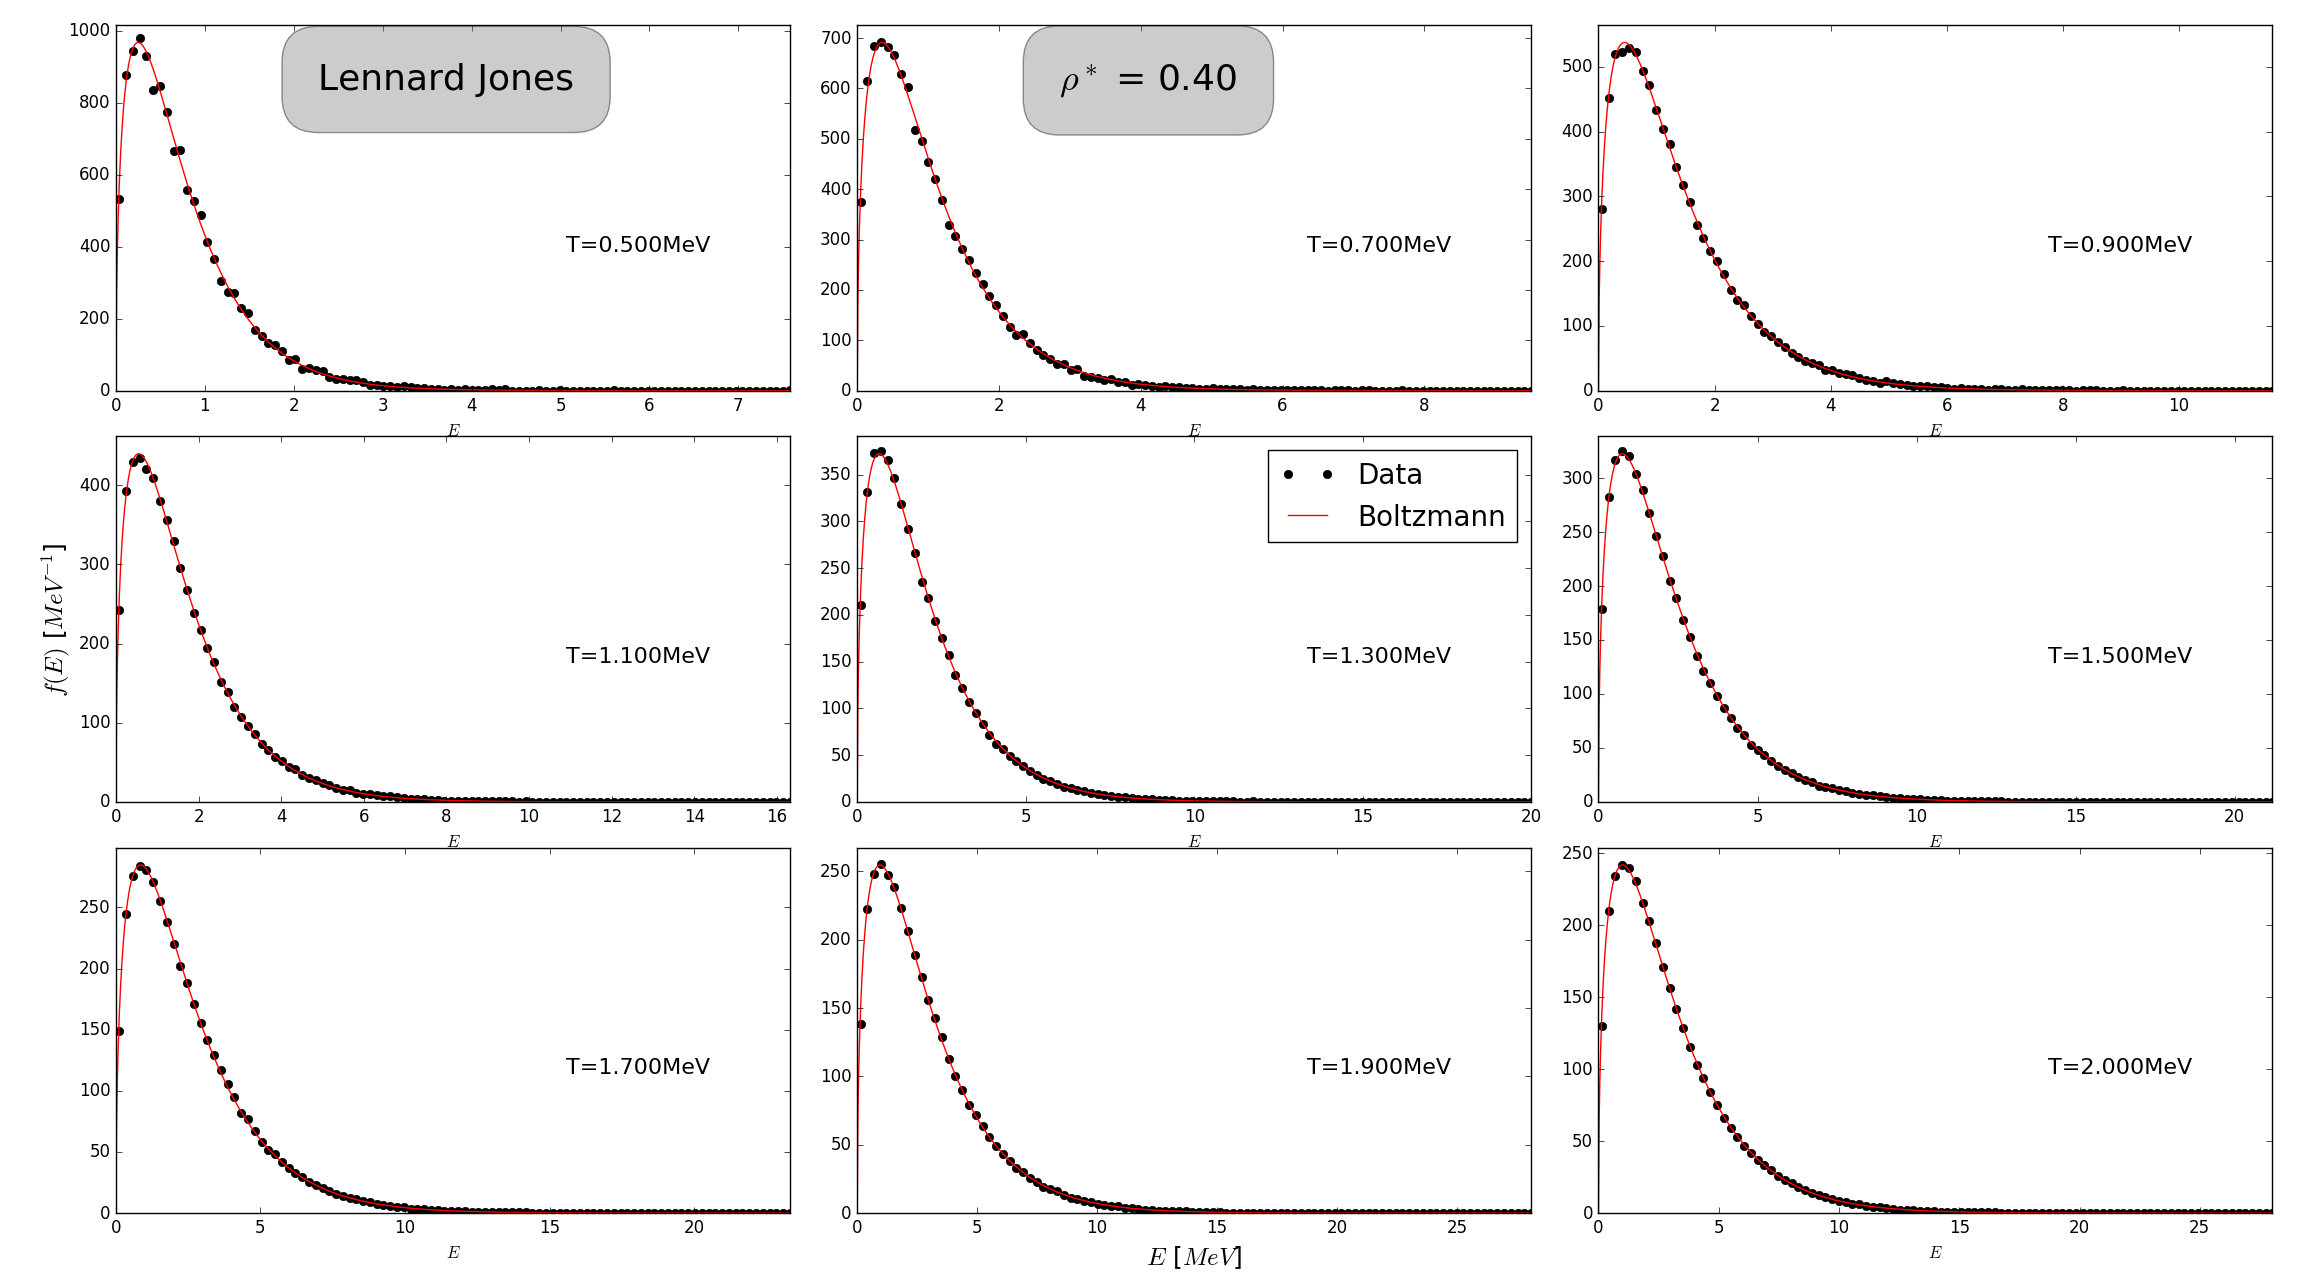
\includegraphics[width=0.9\textwidth]{pauli_gas/histogramas/hist_rho0_LJ.png}
	\caption{Distribuciones de energía cinética para gas de Lennard Jones y $\rho^* = 0.4$.
	La distribución resulta inequivocamente Maxwell-Boltzmann.}
	\label{fig:hist_rho0_LJ}
\end{figure}
\begin{figure}[H]
	\centering
	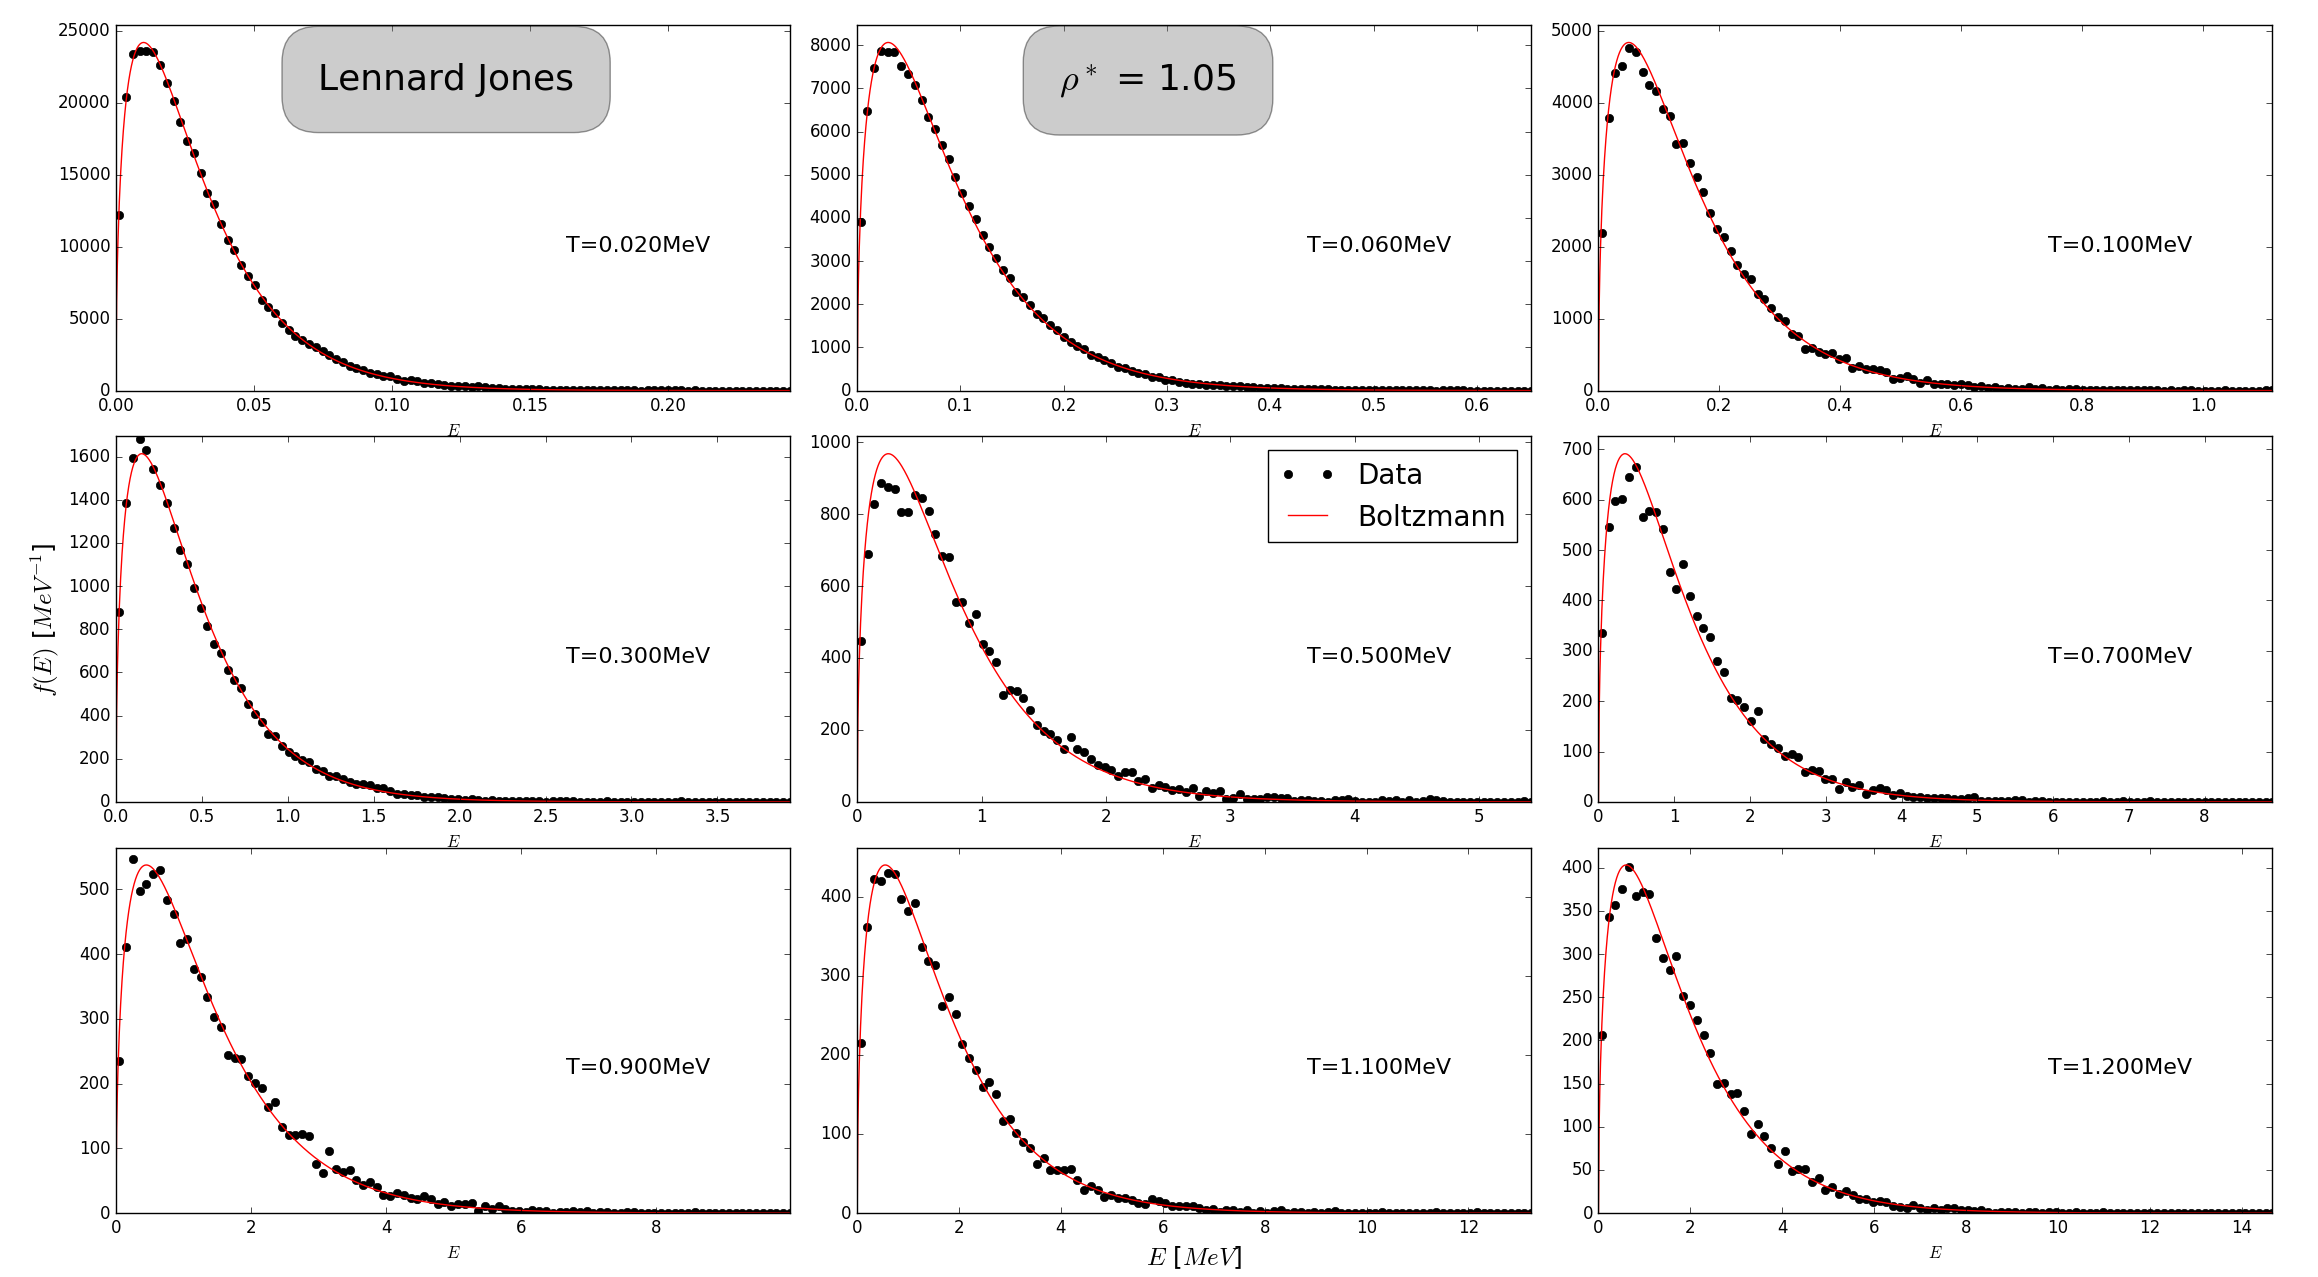
\includegraphics[width=0.9\textwidth]{pauli_gas/histogramas/hist_rho1_LJ.png}
	\caption{Distribuciones de energía cinética para gas de Lennard Jones y $\rho^* = 1.05$.
	La distribución resulta inequivocamente Maxwell-Boltzmann.}
	\label{fig:hist_rho1_LJ}
\end{figure}


\subsection{Temperatura y presión del virial}

A pesar de que nuestras simulaciones de Metropolis-Montecarlo tienen una temperatura $T$ definida, nos resultó razonable analizar si esta coincidia con la temperatura predicha por el teorema del virial.
Utilizamos las 1600 muestras del sistema junto con \eqref{eq:virial_T} para calcular la temperatura del virial $T_V$.
Los resultados para ambos conjuntos de parámetros y las 3 densidades pueden apreciarse en la \textbf{Figura \ref{fig:TvsT_sim}}, donde esta coincidencia se confirma perfectamente.

\begin{figure}[H]
	\centering	%trim={<left> <lower> <right> <upper>}
	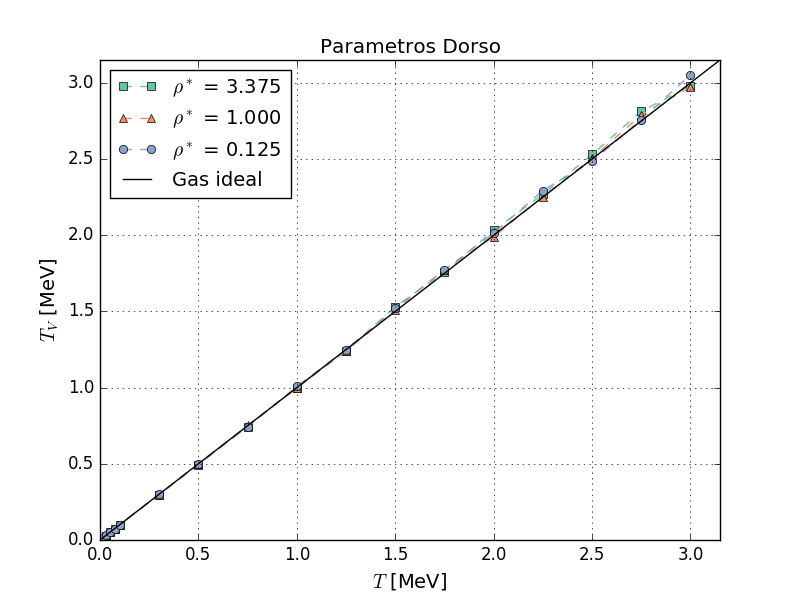
\includegraphics[trim = 5mm 0mm 10mm 5mm, clip, width=0.4\textwidth]{pauli_gas/TvsT_virial_dorso.png}
	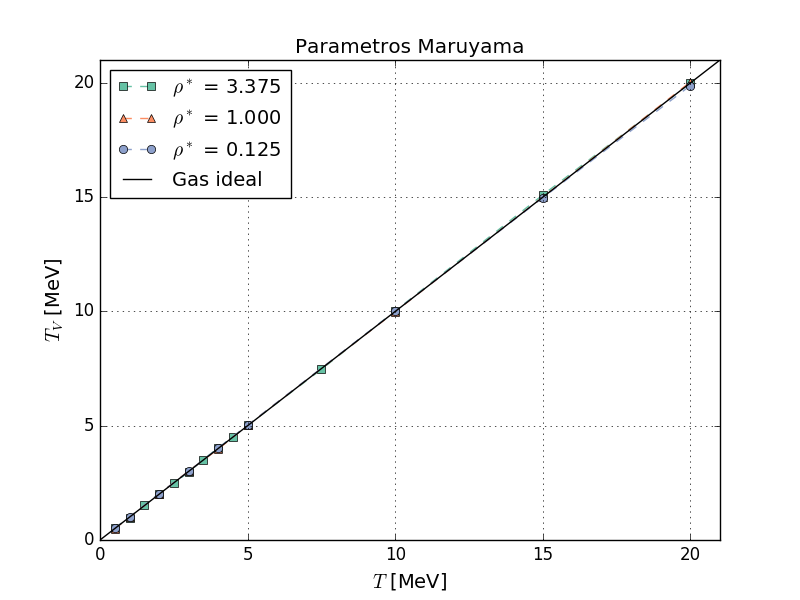
\includegraphics[trim = 5mm 0mm 10mm 5mm, clip, width=0.4\textwidth]{pauli_gas/TvsT_virial_maruyama.png}
	\caption{Graficos de temperatura del virial $T_V$ en función de la temperatura $T$ de la simulación para ambos conjuntos de parametros y las 3 densidades.
	En ambos casos, la coincidencia entre $T_V$ y $T$ es exacta.}
	\label{fig:TvsT_sim}
\end{figure}

Confirmado esto, pasamos al cálculo de la presión para el gas de Pauli utilizando \eqref{eq:virial_P} para ambos conjuntos de parámetros
Graficamos estas presiones para las 3 densidades reducidas en función de la temperatura y las mostramos en la \textbf{Figura \ref{fig:PvsT_sim}}.
Podemos apreciar que ambos conjuntos de parametros arrojan curvas similares (salvo reescalamiento en $T$).

\begin{figure}[H]
	\centering	%trim={<left> <lower> <right> <upper>}
	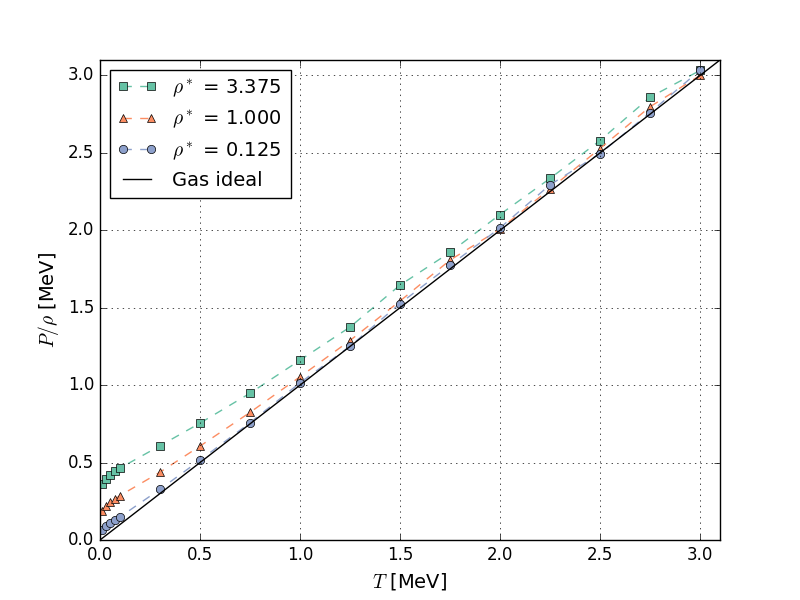
\includegraphics[trim = 5mm 0mm 10mm 5mm, clip, width=0.4\textwidth]{pauli_gas/P_vs_T_dorso.png}
	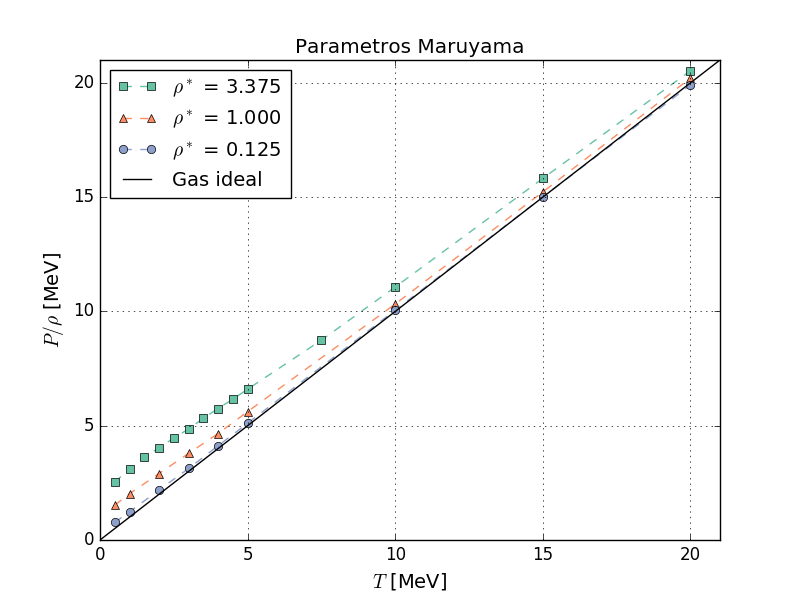
\includegraphics[trim = 5mm 0mm 10mm 5mm, clip, width=0.4\textwidth]{pauli_gas/P_vs_T_maruyama.png}
	\caption{Graficos de presión en función de la temperatura para ambos conjuntos de parametros y las 3 densidades.
	  Salvo el reescalamiento en $T$ resultan muy similares, donde parecería que $P(T=0)\neq0$.}
	\label{fig:PvsT_sim}
\end{figure}

Como es de esperar, la presión coincide con $\rho T$ para $T$ alta y se mantiene levemente por ensima a medida que $T\to0$.
Ciertamente, parecería que $P(T=0)\neq0$, una característica crucial de un gas de fermiones.
